\documentclass{article}

\usepackage{graphicx} % Required for inserting images
\usepackage{amsmath, amssymb}
\usepackage[table]{xcolor} % optional for shading  
\renewcommand{\arraystretch}{1.3} % increase row spacing  
\usepackage{multirow} 
\usepackage{array}  
\usepackage{adjustbox} 
\usepackage{tikz}  
\usetikzlibrary{trees} 
\usepackage{pdflscape}  
\usepackage{float}
\usepackage{geometry}[0.5cm]
\usetikzlibrary{shapes, arrows, calc, positioning, backgrounds, fit} 
\usetikzlibrary{arrows.meta} 
\usepackage[utf8]{inputenc}
\usepackage{tocloft}
\usepackage{titlesec}
\usepackage{fancyhdr}
\usepackage{mdframed}  
\usepackage{listings}  
\usepackage{booktabs}

\newcommand\mymapsto{\mathrel{\ooalign{$\rightarrow$\cr%
  \kern-.15ex\raise.275ex\hbox{\scalebox{1}[0.522]{$\mid$}}\cr}}}

% Define R style  
\definecolor{Rcomment}{RGB}{0,128,0}  
\definecolor{Rstring}{RGB}{128,0,0}  
\definecolor{Rkeyword}{RGB}{0,0,255}  
  
\lstdefinestyle{R}{  
  language=R,  
  basicstyle=\ttfamily\small,  
  keywordstyle=\color{Rkeyword}\bfseries,  
  stringstyle=\color{Rstring},  
  commentstyle=\color{Rcomment}\itshape,  
  numbers=left,  
  numberstyle=\tiny,  
  numbersep=5pt,  
  breaklines=true,  
  showstringspaces=false,  
  frame=single  
}  




% adding a header
\pagestyle{fancy}
\fancyhf{}
\lhead{Superbonus}
\rhead{Henrik Berger, Sara Feore, Romain Fernex, Lauri Hannikainen}
\cfoot{ \thepage}
\renewcommand{\headrulewidth}{0.8pt}

\usepackage[most]{tcolorbox}

\newtcolorbox{simplebox}[1]{  
  title=#1,               % Title from argument  
  colback=blue!10,        % Light blue background  
  colframe=blue!70!black, % Dark blue frame  
  fonttitle=\bfseries,    % Bold title  
  boxrule=0pt,            % No frame around the text area  
  toprule=2mm,            % Thick rule at the top (blue band)  
  enhanced,               % Required for shadow  
  drop shadow             % Simple shadow with default settings  
}  


% Increase TeX memory allocation  
\maxdeadcycles=1000  
\extrafloats{100}  

\title{Superbonus: A Game-Theoretic Analysis}
\author{Henrik Berger, Sara Feore, Romain Fernex, Lauri Hannikainen, }
\date{May 2025}

\begin{document}


% ——— Econometrica‐style front page ———
\begin{titlepage}
  \centering
  % Journal name
  {\Large\scshape Microeconomics II - Game Theory}\\[2cm]
  % Article title
  {\huge\bfseries Superbonus: A Game-Theoretic Analysis}\\[1.5cm]
  % Authors
  {\large  Henrik Berger\quad Sara Feore\quad Romain Fernex \quad Lauri Hannikainen}\\[1cm]
  % Date
  {\large May 2025}\\[2cm]
 


% ——— Abstract ———
\begin{abstract}
 Off-balance sheet fiscal vehicles, such as Italy’s “Superbonus” program, allow governments to hide public debt outside official accounts, complicating the enforcement of fiscal rules. We study how the use of such schemes and coordination between EU member states affect the European Commission’s incentives to enforce fiscal discipline. We develop a game-theoretic signaling model in which a government has private information about whether it is responsible or rent-seeking and chooses whether to report a public debt increase transparently or to conceal it using an off-budget maneuver, while the European Commission decides whether to sanction the government. We then extend this base model in two directions—across time and across countries. First, we consider a two-period setting in which the government’s type can change between periods and the government can choose among transparent borrowing, concealing debt via a Superbonus-style scheme, and no borrowing. We show that, in equilibrium, when enforcement by the Commission is unlikely and sanctions are severe, even a responsible government prefers to hide debt. The likelihood of concealment increases with the severity of sanctions and the perceived leniency of enforcement, and it decreases with higher economic or political costs of hiding debt. Second, we introduce a two-country framework in which governments simultaneously choose debt levels under the threat of proportional sanctions from the Commission. In this setting, each government’s incentive to cooperate with the other country to reduce the overall debt depends on its debt preferences and unequal balance of powers between countries. We find that proportional sanctions induce high-debt weaker countries to cooperate more than low-debt countries. By contrast, under a fixed-penalty regime, sustaining mutual cooperation would require an implausibly high enforcement cost. These results highlight the importance of comprehensive fiscal rules that do not only depend on debt-to-GDP ratio, but take into account differing natures of sovereign liabilities. 
\end{abstract}

\end{titlepage}
\setcounter{page}{1}
% ————————————————————————————

\tableofcontents
\newpage





\section{Introduction}
In economic literature, extensive research has tried to answer how political incentives affect fiscal decisions. Multiple reasons for present-biasedness, a preference structure in which the
government overvalues current spending relative to future welfare compared to society, have been identified. Most prominent reasons include short sightedness (Alesina
and Tabellini, 1990), common pool resource problems (Roubini and Sachs, 1989) and electoral cycles
(Alesina and Sachs, 1988). The issue can be further exacerbated in a monetary union, where a free-riding dynamic exists (Kirchsteiger and Larch, 2023). To mitigate the present bias, countries impose rules on their governments. In the case of the Euro Area, a supranational political entity, the Commission, is responsible of enforcing these rules. 

In the case of the Euro Area, The Stability and Growth Pact (SGP) limits budget deficits to 3 per cent of GDP and debt to 60 per cent of GDP, with the European Commission tasked as the watchdog. In practice, however, member states frequently breach these rules “more by their breach than their observance,” and formal sanctions have never been applied since the SGP’s inception. This track record has undermined the credibility of the fiscal framework. Governments have repeatedly found ways to evade or delay fiscal discipline – from creative accounting tricks to outright collusion in blocking penalties. A recent example is Italy’s “Superbonus” scheme, a generous tax-credit program for home renovations that effectively created a hidden debt burden. Initially expected to cost €35 billion over 15 years, it exploded to almost €150 billion of liabilities in just four years. The Superbonus caused Italy’s deficit to surge to 7.2 per cent of GDP in 2023 (far above the 5.3 per cent without the scheme).

Game-theoretically, the enforcement of the European Union’s fiscal rules is often conceptualized as a strategic game between national governments and the supranational enforcer. In these models, players include a government that decides on fiscal policy (whether to comply with deficit limits or overspend) and an enforcing authority that decides whether to initiate sanctions or leniency. Other frameworks include additional actors, multiple governments or voters, but early theoretical work often simplified enforcement as automatic or driven by voters rather than by a strategic enforcer. Key actions in the game are the government’s budgeting (compliant or violating the rules) and the enforcer’s response (sanction or not). The timing is usually sequential: the government moves (choosing a deficit level or a report), and then the enforcer responds. The information structure is frequently one of incomplete information – the government may have private information about its fiscal situation or type (e.g. whether a deficit breach is due to unavoidable crisis spending or opportunistic overspending). This asymmetry gives a natural rise to signaling games.
 
Early models of fiscal rule compliance often treated enforcement as exogenous or entrusted to the electorate. For example, in “enforcement by voters” models, the public sets a deficit limit and uses elections to punish non-compliant incumbents. In such principal-agent frameworks (e.g. Besley and Smart 2007; Debrun and Kumar 2007; Drazen and Eslava 2005), voters commit to vote out the government if it violates a pre-set budget cap. However, these voter-enforcement models assume that voters can and will reliably act as disciplinarians. In practice, electoral accountability faces problems: voters lack direct tools to enforce fiscal rules and may have difficulty attributing blame for deficits. Empirically, electoral incentives often increase fiscal profligacy rather than enforce discipline. Thus, recent theoretical work shifts focus to the Commission as a strategic enforcer, recognizing that enforcement is a deliberate political act rather than an automatic mechanism.
 
We have identified several papers in the literature with similar modeling decisions. For instance, Wijsman and Crombez (2017) develop a two-period model in which a government can either reveal itself as “undisciplined” by blatantly overshooting deficits, or mimic a “disciplined” government by attributing modest overspending to a high-cost crisis. The Commission, anticipating this behavior, weighs the credibility and cost of enforcement in each case.
 
A key result from this literature is that equilibrium play is “bang bang” (Halac and Yared, 2022). That is, in equilibrium, the government increases debt until a threshold level at which EC is indifferent between punishing and leniency. With this strategy, the EC can achieve the socially optimal outcome under moral hazard. However, this equilibrium does not survive the intuitive criterion, because it hangs on a non-credible off-equilibrium path threat (Kirschteiger and Larch, 2023). Punishing a highly indebted member state makes it even worse off and has high enforcement costs attached to it. Multiple explanations for these high enforcement costs have been proposed, most prominent examples being the risk of “euroskepticism”, and the fact that other countries, that form the EC, often lack incentives to be prudent as they are worried of being next in line if fiscal rules are enforced (Wijsman and Crombez, 2017). 

Moreover, we observe highly indebted countries employing complicated financial vehicles to hide debt off the books, partly because the EGB is ambiguous in its treatment of future liabilities. A prominent example of this is the already infamous “Superbonus”, but other examples include Greece under-reporting its deficit figures prior to the 2009 debt crisis, and Italy engaging in derivatives transactions in the late 1990s and early 2000s to flatter its debt ratio. We call these two observations, enforcement leniency and off the books accounting, the stylized facts of supranational fiscal rules.

In this study we pose the following research question: How off-balance sheet debt vehicles and intergovernmental collaboration affect fiscal rules enforcement? To this end, we develop a novel game-theoretic approach.  Firstly, we propose a signaling game to analyze the strategic interaction between member states and the European Commission (EC) in the enforcement of fiscal rules. Our model demonstrates that when the EC lacks credible and nuanced enforcement mechanisms, both honest and dishonest governments may be incentivized to conceal their fiscal intentions, leading to an increased prevalence of off-balance sheet debt. In particular, indiscriminate or rarely enforced punishments can undermine fiscal discipline by discouraging transparency and encouraging hidden debt strategies.
Secondly, we extend the analysis to consider how a government’s decision to be transparent or conceal debt depends on its expectations about the EC’s enforcement strategy. We show that if the expected punishment is high but enforcement credibility is low, dishonest governments are more likely to hide debt, while honest governments may use transparency as a test of the EC’s stance. This highlights the importance of credible and targeted enforcement for effective fiscal rule compliance.
Finally, we examine the multilateral dynamics that arise when multiple member states coordinate their fiscal actions. Our results indicate that the type and proportionality of penalties chosen by the EC are crucial. Proportional sanctions, which scale with the extent of fiscal violations, can deter breaches more efficiently and at a lower political cost, especially in a context of uneven power among member states. This helps explain observed patterns of enforcement leniency and the persistent use of off-balance sheet debt in the Eurozone.


The remainder of the paper unfolds in three steps. Section 2 develops the foundational signaling game that captures the strategic interaction between a government and the European Commission under asymmetric information. Section 3 extends this framework to a dynamic two-period setting, where governments face evolving incentives and reputational trade-offs over time. Section 4 shifts the lens to a multi-country environment, exploring how intergovernmental dynamics and the structure of sanctions shape collective fiscal behavior. We conclude by discussing the policy implications of our findings for the design of robust and credible fiscal oversight in the European Union.


\section{Base Game : A signaling game of cat and mouse}
We wish to understand the behavior of the EC in response to Italy when Italy has the power to enact a policy similar to the superbonus policy we described above, where it increases its debt but hides it from the EC. As would be the case in the real world, an increase in public spending, transparent or not, contributes negatively to the stability of the Eurozone. We investigate when the EC will impose costly sanctions on Italy, taking into account the risk of punishing it unjustly.  
\subsection{Game description}
\textbf{Structure :} Finite Signaling game\\
\textbf{Course of Play :} Nature attributes a type to Italy (either Honest or Dishonest) which is private informtion to Italy. Then Italy chooses between two actions : communicate that there was an increase in its public spending/debt to the European Commission, or communicate that there was no debt increase. When Italy communicates the latter, the EC does not know if this is indeed the result of a genuine commitment by Italy to not increase its debt, or just the byproduct of a fiscal manipulation to hide an increase in public spending through tax credits (the Superbonus policy). 

\begin{table}[h!]  
\centering  
\renewcommand{\arraystretch}{1.2}  
\begin{tabular}{>{$\displaystyle}l<{$} p{10cm}}  
\toprule  
\textbf{Variables} & \textbf{Description} \\  
\midrule  
S & Economic stimulus and domestic popularity gain that comes with an increase in public spendings \\  
P & Amount of the punishment inflicted by the commission \\  
R   & Credibility and stability gain for the European commission\\  
c & Cost of enforcement i.e cost of punishing a country that does not stay in line with existing fiscal rules (it can be perceived as a political cost for the EC)\\  
$\theta$  & Type of the country (it can be either honest $\theta_H$ or dishonest $\theta_D$ \\  
\bottomrule  
\end{tabular}  
\end{table}  

\subsection{Representation of the game }
In the first period Nature draws the type of Italy following a Bernoulli distribution with parameter $\gamma$. 
\begin{figure}[H]  
\centering  
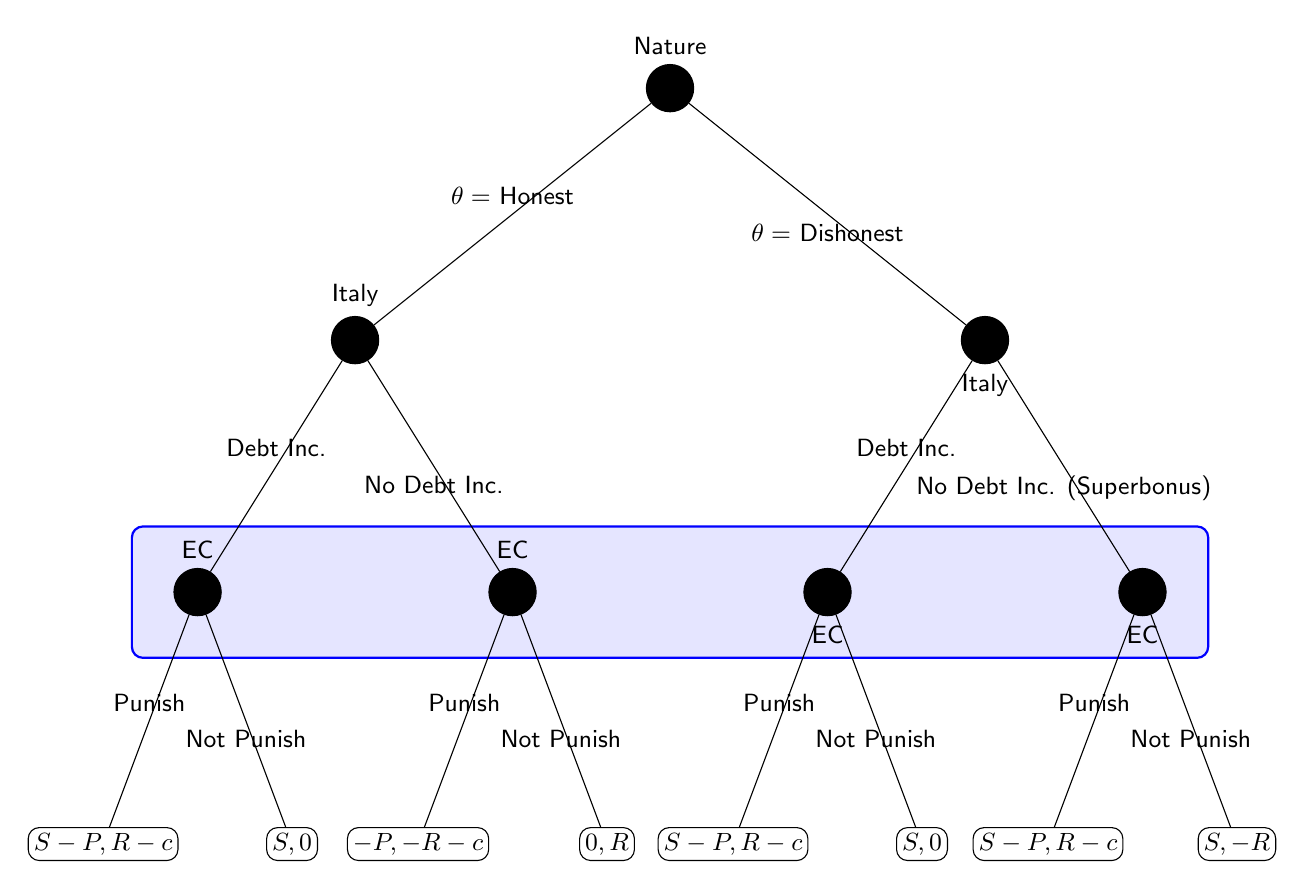
\begin{tikzpicture}[  
    scale=.8,  
    level 1/.style={level distance=4cm, sibling distance=10cm},  
    level 2/.style={level distance=4cm, sibling distance=5cm},  
    level 3/.style={level distance=4cm, sibling distance=3cm},  
    every node/.style={font=\sffamily\small},  
    main node/.style={circle, draw, fill=black, inner sep=1.5pt, minimum size=6mm},  
    terminal node/.style={rectangle, draw, inner sep=2pt, rounded corners},  
    branch label/.style={midway, fill=white, inner sep=1mm},  
    grow=down  
]  
% Root node (Nature)  
\node[main node, label=above:Nature] (Nature) {}  
    child {  
        node[main node, label=above:Italy] (ItalyH) {}  
            child {  
                node[main node, label=above:EC] (EC_H_Inc) {}  
                    child {  
                        node[terminal node] {$S-P, R-c$}  
                        edge from parent node[above] {Punish}  
                    }  
                    child {  
                        node[terminal node] {$S,0$}  
                        edge from parent node[below] {Not Punish}  
                    }  
                edge from parent node[above] {Debt Inc.}  
            }  
            child {  
                node[main node, label=above:EC] (EC_H_No) {}  
                    child {  
                        node[terminal node] {$-P,-R-c$}  
                        edge from parent node[above] {Punish}  
                    }  
                    child {  
                        node[terminal node] {$0, R$}  
                        edge from parent node[below] {Not Punish}  
                    }  
                edge from parent node[below] {No Debt Inc.}  
            }  
        edge from parent node[above] {$\theta =  $ Honest}  
    }  
    child {  
        node[main node, label=below:Italy] (Italy) {}  
            child {  
                node[main node, label=below:EC] (EC_D_Inc) {}  
                    child {  
                        node[terminal node] {$S-P,R-c$}  
                        edge from parent node[above] {Punish}  
                    }  
                    child {  
                        node[terminal node] {$S,0$}  
                        edge from parent node[below] {Not Punish}  
                    }  
                edge from parent node[above] {Debt Inc.}  
            }  
            child {  
                node[main node, label=below:EC] (EC_D_No) {}  
                    child {  
                        node[terminal node] {$S-P, R-c$}  
                        edge from parent node[above] {Punish}  
                    }  
                    child {  
                        node[terminal node] {$S, -R$}  
                        edge from parent node[below] {Not Punish}  
                    }  
                edge from parent node[below] {No Debt Inc. (Superbonus)}  
            }  
        edge from parent node[below] {$\theta= $ Dishonest}  
    };  
% Blue box spanning across the EC nodes  
\begin{scope}[on background layer]  
    \node[fit=(EC_H_Inc)(EC_H_No)(EC_D_Inc)(EC_D_No), inner sep=15pt, fill=blue!10, draw=blue, thick, rounded corners] {};  
\end{scope}  
\end{tikzpicture}  
\caption{payoffs : S is the gain from the debt increase, P the amount of the punishment, c the cost of enforcement, R the reputation benefit for the EC (enforcing fiscal rules might deter breaches in the future).}  
\end{figure}  

\textbf{Parametric Assumptions : }
\begin{itemize}
    \item We assume $R>c$, i.e., that the gain in stability from punishing an increase in debt more than offsets the enforcement cost for the EC. This follows from the fact that we only consider debt increases that are above the threshold "bang bang" proposed by Halac and Yared (2022). Thus, the analysis does not apply to small increases in debt. 
\end{itemize}
\subsection{Deriving the model}
\subsubsection{Separating Equilibria}
Now that we have described this signaling game, we begin by solving for separating equilibria.\\
\indent \textbf{Case 1 : } 
Strategy : $\theta_D$ always plays ND and $\theta_H$ always plays D
We consider the following conditional conditional probabilities : 
\begin{equation}
\left\{
\begin{aligned}
    &P(\theta_D|m_{debt}) = \mu_D = 0 \\
    &P(\theta_D|m_{nodebt})= \mu_{ND}=1-\mu_D=1
\end{aligned}
\right.
\end{equation}
After considering expected payoffs for the EC we determine that it will punish Italy both when it receives $m_{debt}$ and when it receives $m_{nodebt}$. 
\begin{equation}
\left\{
\begin{aligned}
    &U_{EC}(P|m_{debt)}>U_{EC}(NP|m_{debt}) \\
    &U_{EC}(P|m_{nodebt}) > U_{EC}(NP|m_{nodebt})
\end{aligned}
\right.
\end{equation}
We find no off-equilibrium path deviations either when punishment is prohibitive ($P>S$) nor when punishment is lax ($P<S$).
Thus we have the following separating PBE : $$PBE :\left\{(m_{debt,\theta_H}, m_{nodebt,\theta_D})(P_{EC},P_{EC}),\mu_D=0,\mu_{ND}=1 \right\}$$

\begin{simplebox}{Proposition 1.1}
In a separating equilibrium with strategy profiles
\( s_{\theta_D}(ND),\ s_{\theta_H}(D) \), we have have a PBE: 

$$\left\{(m_{debt,\theta_H}, m_{nodebt,\theta_D})(P_{EC},P_{EC}),\mu_D=0,\mu_{ND}=1 \right\}$$
\end{simplebox}

Since the honest type cannot use Superbonus to hide debt, it has no incentive to deviate from a transparent debt increase. Similarly, since the dishonest type knows that it will get punished whenever it increases debt, there is no incentive for it to deviate. 

\textbf{Case 2 : }
The strategy of Italy now shifts to : $\theta_D$ always plays $m_{debt}$ and $\theta_H$ always plays $m_{nodebt}$.
The conditional probabilities inferred by the EC are now : 
\begin{equation}
\left\{
\begin{aligned}
    &\mu_D = 1 \\
    &\mu_{ND}=1-\mu_D=0
\end{aligned}
\right.
\end{equation}
In this new setting, the EC prefers to punish when it sees $m_{debt}$ but would rather not punish when it sees $m_{nodebt}$ to avoid punishing an innocent. \\
However, when checking for off equilibrium deviations, it is clear that a dishonest Italy will capitalize on the EC's belief to play superbonus and get $S$ instead of $S-P$. This is true both when $S>P$ and when $S<P$.
\begin{simplebox}{Proposition 1.2}
If the EC is naïve (believes that Italy will commit to its equilibrium actions regardless of its type), Italy, if dishonest, will wish to exploit this weakness to improve its gain by concealing its debt increase. 
\end{simplebox}

\subsubsection{Pooling Equilibria}
We now consider cases where both types of Italy opt for the same action in equilibrium which prevents the bayesian updating that the EC benefited from earlier. \\
\indent \textbf{Case 1 : }
Both types of Italy play $m_{debt}$, which implies the following conditional probabilities : 
\begin{equation}
\left\{
\begin{aligned}
    &\mu_D = \gamma\\
    &\mu_{ND}=arbitrary
\end{aligned}
\right.
\end{equation}
We can now compute the expected payoff for the EC to find 1) the action the EC will want to play when it receives $m_{debt}$ and 2) find a threshold value for $\mu_{ND}$ :\\
Firstly, we get :
\begin{equation}
\begin{aligned}
    &U_{EC}(P|m_{debt})=\mu_D(R-c)+(1-\mu_D)(R-c)=R-c>0\\
    &U_{EC}(NP|m_{debt})=\mu_D\times0+(1-\mu_D)\times0=0
\end{aligned}
\end{equation}
As expected, when the EC receives $m_{debt}$ its preferred action does not depend on $\mu_D$ and it will always prefer to punish. Now let us compute the payoffs conditional on $m_{nodebt}$ : 
\begin{equation}
\begin{aligned}
    U_{EC}(P|m_{debt})&=\mu_{ND}(R-c)+(1-\mu_{ND})(-R-c)\\
    &=R\mu_{ND}-c\mu_{ND}-R-c+R\mu_{ND}+c\mu_{ND}\\
    &=2R\mu_{ND}-R-c\\
    U_{EC}(NP|m_{debt})&= \mu_{ND}(-R)+(1-\mu_{ND})R\\
    &=-2R\mu_{ND}+R
\end{aligned}
\end{equation}
We solve for the threshold value $\mu_{ND}^*$ using the indifference condition:
\begin{equation}
\begin{aligned}
    2R\mu_{ND}^*-R-c&=-2R\mu_{ND}^*+R\\
    4R\mu_{ND}^*&=2R+c\\
    \mu_{ND}^*&=\frac{2R+c}{4}
\end{aligned}
\end{equation}
Let's start by looking at the case when $\mu_{ND}>\mu_{ND}^*$: we have
\begin{equation}
    U_{EC}(NP|m_{nodebt})<U_{EC}(P|m_{nodebt})
\end{equation}
The EC prefers to punish when receiving $m_{nodebt}$. We find no profitable deviation off the equilibrium path thus this is a Pooling PBE.
$$PBE : \left\{ (m_{debt,\theta_D},m_{debt,\theta_{ND}}),(P_{EC},P_{EC}),\mu_D=\gamma,\mu_{ND}>\mu_{ND}^*\right\}$$
\begin{simplebox}{Proposition 1.3}
    When the probability of dishonest is too high both players end up increasing their debt to avoid unjust punishment. The honest player is too scared of being targeted by accident which leads to a situation that is highly suboptimal for the Eurozone as countries prefer going into debt rather than keeping a sound financial situation. 
\end{simplebox}
Now, we look at the case when $\mu_{ND}<\mu_D$. In this case the EC prefers not to punish when it receives $m_{nodebt}$. \\
This means there exists a profitable off equilibrium deviation for type $\theta_D$ as it can now safely go for superbonus without fearing punishment.\\ 
\indent\textbf{Case 2 : }
Both types of Italy play $m_{nodebt}$. Thus, we have: 
\begin{equation}
\left\{
\begin{aligned}
    &\mu_D = arbitrary\\
    &\mu_{ND}= \gamma
\end{aligned}
\right.
\end{equation}
As in case 1, we first compute the payoffs for the EC :
\begin{equation}
\left\{
\begin{aligned}
    &U_{EC}(P|m_{debt})=R-c\\
    &U_{EC}(NP|m_{debt})=0
\end{aligned}
\right.
\end{equation}
We notice that the payoffs for the EC off the equilibrium path are not dependent on $\mu_{ND}$ so we do not need to look for a threshold value for off equilibrium probabilities like we did in case 1. 
\begin{equation}
\left\{
\begin{aligned}
    &U_{EC}(P|m_{nodebt})=\gamma(R-c)+(1-\gamma)(-R-c)=2R\gamma-R-c\\
    &U_{EC}(NP|m_{nodebt})=\gamma(-R)+(1-\gamma)R = R-2R\gamma
\end{aligned}
\right.
\end{equation}
This time, which action will be preferred by the EC when receiving $m_{debt}$ depends on $\gamma$ (so on $\mu_{ND}$), so we do need to consider the threshold value for this variable. The EC punishes Italy when : 
\begin{equation}
\begin{aligned}
    2R\gamma-R-c>R-2R\gamma\\
    \gamma >\frac{2R+c}{4R}
\end{aligned}
\end{equation}
When this condition is satisfied, the EC punishes in every situation so an honest Italy will want to switch to increasing its debt as it would get $S-P$ instead of $-P$. We have a profitable off equilibrium deviation for the honest type. \\
But now let us suppose this condition is not satisfied: the EC will not punish when receiving $m_{nodebt}$ so there exists no profitable deviation for either player (superbonus works so there is no need to be transparent).
\begin{equation}
    \text{PBE : } \left\{(m_{nodebt,\theta_H}, m_{nodebt,\theta_D})(NP_{EC},P_{EC}),\mu_D\in
[0,1],\mu_{ND}=\gamma<\frac{2R+c}{4R} \right\}
\end{equation}
\begin{simplebox}{Proposition 1.4}
    When the enforcement cost is high, even if the probability of Italy being dishonest is high as well the EC is likely to get cold feet and avoid punishing altogether. Conversely, when the benefit R of punishing is high, the EC will be more willing to opt for preemptive punishment. 
\end{simplebox}

\subsection{Key Takeaways}

\textbf{Separating equilibrium:}
We find one separating equilibrium. In the first case, an honest government increases debt transparently and a dishonest government government chooses to hide. Thus, the EC chooses to punish in all nodes. \\

\textbf{Pooling equilibria :}
We find two pooling equilibria. 
When both countries send transparent debt increases, the EC chooses to punish in all nodes. The dishonest type is indifferent between superbonus and a transparent increase in debt, thus there are no profitable deviations. Not knowing the probability of dishonesty, the EC would prefer to punish them anyway if they sent a no-debt increase message. Secondly, when both countries increase debt transparently, punishment will depend on the EC's enforcement cost. If the EC's cost is low, it will punish in all nodes, and conversely, if they are high, the EC will avoid punishing (even with a high probability of dishonesty). \\


 We showed that when the EC operates based on a naïve belief system (assumes the odds of Italy cheating are close to none) this creates a strong incentive for fiscal manipulation by a dishonest government. Conversely, should the EC assume Italy is always trying to deceive it and punish Italy regardless of its action, this will prompt a welfare diminishing outcome where Italy prefers to increase its debt regardless of its type. In other words this excessive reliance on punishment without adequate informational foundations undermines the fiscal discipline such policies are intended to promote. This mechanism, however, seems fairly disconnected from reality as the EC tends to be significantly more fearful of inflicting punishment and would most likely never take the risk of punishing a country even when presented with significant evidence, absent popular support. This politically grounded non-credibility is studied extensively in the first extension below which looks at the problem from the perspective of Italy. 



\section{Extension n°1 : To hide or not to hide ? - Italy's perspective}
\subsection{Game description}
We consider the same two players as in our base game, Italy and the European commission. We now position ourselves from Italy's perspective and try to understand what might prompt Italy to play superbonus and to what extent Italy might be willing to bet on the inertia of the Commission to increase its payoffs. Compared to the first game, we make the choice to be significantly more conservative regarding the odds of the EC punishing Italy, but keep the idea of prohibitive punishment ($P>S$). To study Italy's behavior, we depart from the base game to introduce the following elements : 
\begin{itemize}
    \item The new game is repeated twice to better understand how Italy might behave when it needs to consider what happens at the next period. 
    \item The type of Italy ($\theta_D,\theta_H$) is drawn twice (once at the beginning of each period) to model the fact that Italy needs to compose with the fact that the reality it is facing might change from one period to the next (due to political factors for instance). We denote $\theta^i$ the type of italy for period $t\in[1,2]$ : 
    \begin{equation}
        \forall t\in[1,2], \theta^t\sim Ber(\mu)
    \end{equation}

    \item Italy, regardless of its type, can now play either of three possible options : increase its debt transparently, increase is debt via off balance sheet vehicles (Superbonus) or not increase its debt. The Superbonus policy is now considered a form of jamming as it prevents the EC from taking action (for fear that it might punish Italy unjustly) but comes with a \textbf{dishonesty cost, H}, if Italy's type for the round considered is $\theta_H$. The intuition is that fiscally responsible governments face reputational costs associated with dishonesty. These include possible judicial penalties for politicians or a fear of public backlash against governments that try to portray themselves as being trustworthy. Dishonest, rent-seeking governments do not care about such consequences.
    
    \item EC has a non null probability $\gamma$ of being a "coward" and never punish Italy regardless of the period or Italy's action. Otherwise, the EC acts based on the payoff matrix shown below. 
\end{itemize}
We make the following assumptions regarding the payoffs for this game : 
\begin{itemize}
    \item We denote $c(\theta)$ the cost of dishonesty with $c(\theta_D)=0$ and $c(\theta_H)=H>0$
    \item For Italy, we assume $S-P<0<S-H<S$
    \item For the EC we assume : $R>c$
\end{itemize}
\subsection{Representation of the game}
\begin{table}[h!]  
\centering  
$$\begin{array}{c|cc}  \text{Italy} \backslash \text{EC} & \text{Punish} & \text{Not Punish} \\  \hline  \text{Debt (Superbonus)} & (S-c(\theta^t), 0) & (S-c(\theta^t), 0) \\  \text{Debt (Transparent)} & (0, -c) & (0, 0) \\  \text{No Debt} & (S-P, R-c) & (S, 0) \\\end{array}$$  
\caption{Matrix of the simultaneous game at period t}  
\end{table}  

\subsection{Deriving the model}
Now that the game has been set, let us consider what Italy will play depending on the following three scenarios : 
\begin{itemize}
    \item When $P(\theta^1=\theta_D)=1$ (Italy is dishonest for sure in the first period)
    \item When $P(\theta^1=\theta_D)=0$ (Italy is honest for sure in the first period)
    \item When $P(\theta^1=\theta_D)=\mu\in]0,1[$ (Italy has a non pull probability $\mu$ of being dishonest in the first period)
\end{itemize}
\subsubsection*{Case 1 : $P(\theta^1=\theta_D)=1$}
Italy is faced with 3 separate options for period 1 : 1) Increase its debt in a transparent way to gauge the type of the EC, 2) Play superbonus and avoid punishment for this period for sure but remain ignorant about the type of the EC, or 3) Not increase its debt and get nothing for sure. \\
Let us compute expected payoffs if Italy plays option 1) or option 2) while accounting for potential future payoffs in period 2. Note that in the case of option 1, the type of the EC is fully revealed for the next period since a rational Italy will always punish in this situation. 
\begin{equation}
\begin{aligned}
    \text{payoff of option 1 (transparency) }&= \gamma(S+S) + (1-\gamma) [(S-P)+S-c(\theta_i^1)]\\
    &=2\gamma S+(1-\gamma)[2S-P-(1-\mu)H]\\
    &=2\gamma S+2S-P-(1-\mu)H-2\gamma S+\gamma P+\gamma(1-\mu)H\\
    &=2S+\gamma P-P-(1-\gamma)(1-\mu)H
\end{aligned}
\end{equation}
For option 2 (hiding), Italy gets no information about the EC for the next period and will therefore want to pick the action with the highest expected payoff for the second period. 
\begin{equation}
\text{payoff of option 2 (hiding) }=S+
\left\{
\begin{aligned}
     &S-(1-\mu)H \text{ if chooses superbonus}\\
     &\gamma S+ (1-\gamma)(S-P) \text{ if chooses transparent increase}\\
     &0 \text{ if chooses not to increase debt}
\end{aligned}
\right.
\end{equation}
Italy will increase its debt transparently at $t=1$ only if the following three conditions are met : 
\begin{equation}
\begin{aligned}
    &\text{payoff(option 1)}>\text{payoff(option 2 $\cap$ superbonus)}\\
    &\text{payoff(option 1)}>\text{payoff(option 2 $\cap$ debt increase)}\\
    &\text{payoff(option 1)}>\text{payoff(option 2 $\cap$ no debt increase)}
\end{aligned}
\end{equation}
Let us check if the second inequality holds : 
\begin{equation}
\begin{aligned}
    2S+\gamma P-P-(1-\gamma)(1-\mu)H&>S+\gamma S+S-P-\gamma S+\gamma P\\
    2S+\gamma P-P-(1-\gamma)(1-\mu)H &> 2S-P+\gamma P\\
    -(1-\gamma)(1-\mu)H&>0
\end{aligned}
\end{equation}
This is impossible since $H>0$, in other words, Italy will always play superbonus in the first game if it is dishonest with certainty. We can now find which condition we can impose on the parameters for Italy to play superbonus in the second period as well : 
\begin{equation}
\left\{
\begin{aligned}
    &S-(1-\mu) H>\gamma S+(1-\gamma)(S-P) \Leftrightarrow H<\frac{1-\gamma}{1-\mu}P\\
    &S-(1-\mu) H>0\Leftrightarrow H<\frac{S}{1-\mu}
\end{aligned}
\right.
\end{equation}
\begin{simplebox}{Proposition 2.1}
    For $P(\theta^1=\theta_D)=1$, Italy will find it optimal to play Superbonus in both periods iff   $H<min(\frac{S}{1-\mu},\frac{1-\gamma}{1-\mu}P)$.
\end{simplebox}

In other words, the probability of superbonus is increasing in the severity of punishment (P), gain from superbonus (S), and odds of the EC not being a "coward" ($1-\gamma$), and decreasing in the cost associated with dishonesty (H). The intuition behind this result is that when a rent-seeking government is in power in the first period, the type of EC is unknown, and in the second period, Italy will weigh the gains from hidden debt versus the probability-weighted severity of punishment. Thus, to discourage hiding debt, a policy maker might find it optimal to set the punishment P at a lower value, or to zero altogether, than absent the possibility of facing a rent-seeking government. Alternatively, increasing the cost of off-balance sheet vehicles (H), e.g. through increased monitoring of member states, can discourage "fiscal gimmickry".  

\subsubsection*{Case 2 : $P(\theta^1=\theta_D)=0$}
We now set the type for period 1 to honest for sure. Let us see if there exists cases where Italy will still play superbonus in the first period despite facing a cost for behaving in a dishonest way.
The payoff of option 1 (transparency) remains unchanged as it is not dependent on Italy's type. \\
We compute payoffs for option 2 again and get : 
\begin{equation}
\text{payoff of option 2 (hiding) }=S-H+
\left\{
\begin{aligned}
     &S-(1-\mu)H \text{ if chooses superbonus}\\
     &\gamma S+ (1-\gamma)(S-P) \text{ if chooses transparent increase}\\
     &0 \text{ if chooses not to increase debt}
\end{aligned}
\right.
\end{equation}
Let us check whether the three conditions we stated for case 1 are valid here : We begin by checking that \text{payoff(option 1)}$>$\text{payoff(option 2 $\cap$ superbonus)}
\begin{align*}  
&2S + \delta P - P - (1-\gamma)(1-\mu)\,H   
   > S - H + \gamma S + (1-\gamma)(S - P) \\[6pt]  
&\qquad\Leftrightarrow (1-\gamma)(1-\mu)\,H < H   
   \quad \text{this is always true!}  
\end{align*}
The first inequality is always verified meaning Italy will never play superbonus twice in this new configuration of the game. We check whether the second condition, \text{payoff(option 1)}$>$\text{payoff(option 2 $\cap$ debt increase)}, is satisfied : 
\begin{align*}
&2S + \gamma P - P - (1-\gamma)(1-\mu)\,H   
   > S - H + S - (1-\mu)\,H \\[6pt]  
&\gamma P - P - (1-\gamma)(1-\mu)\,H   
   > (\mu - 2)\,H \\[6pt]  
&\gamma P - P   
   > \bigl[(\mu - 2) + (1-\gamma)(1-\mu)\bigr]\,H \\[6pt]  
&\gamma P - P   
   > \bigl[\mu - 2 + 1 - \mu - \gamma + \gamma\mu\bigr]\,H \\[6pt]  
&\gamma P - P   
   > (\gamma\mu - \gamma - 1)\,H  \\[6pt] 
& H>\frac{(\gamma-1)P}{(\gamma \mu-\gamma-1)}>0
\end{align*}  
\begin{simplebox}{Proposition 2.2}
If the cost of dishonesty is high enough, $H>\frac{(\gamma-1)P}{(\gamma \mu-\gamma-1)}$, Italy will place a higher value on figuring out the Commission's type. Feeling the waters is indeed a safer strategy for Italy in this case because the benefits of the superbonus in the second period are too low. Should the cost of dishonesty be sufficiently low, however, even if Italy is honest for sure in the first period it will end up playing superbonus in the first period.
\end{simplebox}
\subsubsection*{Case 3 : $P(\theta^1=\theta_D)=\mu\in]0,1[$}
The payoff of playing superbonus at t=1 is now : 
\begin{equation}
\text{payoff of option 2 (hiding) }=S-(1-\mu)H+
\left\{
\begin{aligned}
     &S-(1-\mu)H \text{ if chooses superbonus}\\
     &\gamma S+ (1-\gamma)(S-P) \text{ if chooses transparent increase}\\
     &0 \text{ if chooses not to increase debt}
\end{aligned}
\right.
\end{equation}
We follow the same procedure as with the previous two cases and get the following conditions : 
\begin{equation}
\left\{
\begin{aligned}
    &\frac{\gamma P-P}{\mu-1+(\mu-1)\gamma}<H\\
    &(1-\gamma)H<H \text{ $\Rightarrow$ always true ! }
\end{aligned}
\right.
\end{equation}
Looking at the first condition we see the decision taken by Italy at t=1 will depend on H and other parameters as was observed in case 2. 
\begin{simplebox}{Proposition 2.3}
    The decision of Italy, when there is uncertainty about its type as soon as the first period, is highly dependent on $\gamma$, the chance that the EC is actually a coward. We provide a detailed analysis of comparative statics for the inequality in case 3 below. 
\end{simplebox}

\subsection{Parameter Sensitivity Analysis and Comparative Statics}
We denote $H^*\equiv f(\gamma,\mu,P)=\frac{\gamma P-P}{\mu-1+(\mu-1)\gamma}$ the threshold value for the cost of dishonesty. In this section we look into how the parameters $\gamma,\mu$ and $P$ influence the value of this threshold. The lower this threshold is, the more likely Italy will decide to be transparent in the first period instead of playing superbonus. 
Looking at the derivatives of f, we can assert the following : 
\begin{itemize}
    \item Holding $\mu$ and $\gamma$ fixed, an increase in the punishment amount raises the odds of Italy playing the superbonus at t=1 since experimenting to see whether the EC is a coward or not is riskier. This implies that imposing a tougher punishment for a debt increase disincentivizes Italy to behave in a transparent way.
    $$\text{partial effect of P} :\frac{\partial f}{\partial P} = \frac{\gamma - 1}{(\mu - 1)(1 + \gamma)} $$
    \item Similarly, holding $\gamma,P$ and $\mu$ itself fixed, we can establish that $\mu$ influences f positively. This means that when Italy is very likely to be dishonest, it prefers playing superbonus at t=1. Besides, f is convex in $\mu$ meaning even a limited increase in $\mu$ can sharply the preference of Italy for playing the superbonus. 
        $$\text{partial effect of $\mu$} : \frac{\partial f}{\partial \mu} = -\frac{P(\gamma - 1)}{(1 + \gamma)(\mu - 1)^2}  $$
    \item The partial effect of $\gamma$ is ambiguous as its sign depends on the relation between $\mu$ and $\gamma$ itself. The convexity of f in $\gamma$, however, is verified for any combination of parameters. A more detailed analysis is provided below. 
    $$\text{partial effect of $\gamma$} : \frac{\partial f}{\partial \gamma} = \frac{P \left[ (\mu - 1) - (\gamma - 1) \right]}{(\mu - 1)(1 + \gamma)^2}  $$
\end{itemize}

\begin{figure}[H]  
    \centering  
    \includegraphics[width=0.9\textwidth]{Graphs/MCS.png}  
    \caption{Comparative statics for the threshold value $H^*$($\equiv f(\gamma,\mu,P))$}  
\end{figure} 
\textbf{Detailed analysis of comparative statics : }
\begin{itemize}
    \item moderating effect of P (magnitude of punishment) : In the bottom left corner we see that the submodularity of f in $(\gamma,P)$ is highly dependent on the value of $\mu$. When the probability of dishonesty is low, P actually reinforces the impact of $\gamma$ on f. Whereas, when $\mu$ is high, the effect of $\gamma$ on f is strongly dampened when the punishment cost rises. Additionally, based on the graph in the bottom left corner, we see that f is submodular in $(P,\mu)$ for any value of $\gamma$, meaning Italy cares more about its probability of begin dishonest at t=1 when the value of punishment is high.  
    \item moderating effect of $\mu$ (likelihood of being dishonest) : Looking at the top-center graph we can see that f is strongly submodular in $(\gamma,\mu)$ which means that as $\mu$ gets closer to 1 the impact of $\gamma$ on f becomes significantly weaker. In other words, when the odds of Italy being dishonest are high, whether the EC has a high chance of being a coward or not is less relevant in Italy's decision to play superbonus or not. Conversely, looking at the top right corner, f is supermodular in $(P,\gamma)$ which implies that the more likely Italy is dishonest the more its decision to play superbonus will be sensitive to the magnitude of the punishment. 
    \item moderating effect of $\gamma$ (likelihood of being a coward) : Based on the partial of f in $\gamma$ we introduced earlier, f depends positively on $\gamma$ only when $\mu<\gamma$. That is when the probability of Italy being dishonest is overshadowed by the probability of the EC being a coward. Unless this is the case, $\gamma$ will actually have the opposite effect and prompt Italy to be more transparent when $\gamma$ grows. 
\end{itemize}

\begin{figure}[H]  
    \centering  
    \includegraphics[width=0.6\textwidth]{Graphs/3DGraph.png}  
    \caption{Representation of the threshold value $H^*$ as a function of $P$ and $\gamma$ for $\mu=0.1$}  
\end{figure}  

\begin{simplebox}{Proposition 2.4}
\begin{enumerate}
    \item Raising penalties for hidden debt can be effective, but only if enforcement is credible ($\gamma$ is low). If the EC is perceived as unlikely to punish, increasing P alone will not lead to a better outcome.
    \item The credibility of the EC (lower $\gamma$) has a genuine deterrent effect on Italy's behavior and can, under the right circumstances, help prevent hidden debt vehicles. 
    \item If the probability of EC being credible is high, a higher punishment intensity (higher P) may backfire by encouraging Italy to “test” the system.
\end{enumerate}
\end{simplebox}

\subsection{Key Takeaways}

In summary, we have shown that the likelihood of Italy playing superbonus is linked to the assumption Italy makes on the credibility of the EC and on the magnitude of the punishment. A key result is that the intensity of the punishment has differing implications for the likelihood of Italy playing superbonus. In fact, when the tendency of the EC to enforce its fiscal rules is low, a higher P incentivizes Italy to hide its debt. This is because when the payoff from a transparent debt increase is low enough (when P is high), hiding debt becomes a dominant strategy. This is not the case when P is low enough. For a low value of P, Italy finds it optimal to decrease the rate at which it hides debt, as the profitability of a transparent debt increases. 

However, one significant limit of this model is that the EC has a clear incentive to punish transparent increases in debt, since the cost of enforcement is fairly low. Therefore, the model has difficulties capturing enforcement leniency present in the data. To better understand this, we now turn to a setting with multiple countries negotiating on their desired level of debt with the EC acting only as the enforcer of last resort. The intuition is that countries often get together to increase the enforcement costs faced by the EC to avoid any form of punishment altogether. This dynamic is also present in the recursive collaboration model that we propose in the appendix.



\section{Extension n°2: The right punishment }

\subsection{Game Description}

In our second extension we are shifting our focus from the interaction between the EC and a single member state to a slightly different setting with multiple member states. This is because fiscal rules are often upheld in less formal negotiations between the member states. The key idea is to highlight the important power imbalances present in the EU. We show that these imbalanced affect incentives to cooperate, and study why the type of punishment given by the EC matters. \\

There are three main participants in this game:

\begin{itemize}

    \item \textbf{The European Commission (EC):} The EC acts as a regulator and can punish the countries if their combined debt level exceeds 4 (this threshold is arbitrary and chosen for illustration purposes). The threshold reflects the tradeoff faced by the EC. The EC, since it represents the member states, faces both the political costs of punishing countries, and the cost linked to the European Central Bank (ECB) raising interest rates after the fiscal stance is too accomodative. The EC's utility is thus both a function of $-\gamma$ (the lower, the less political cost) and of the probability of the total level of debt exceeding 4 (the lower, the better).
    To start, the punishment is proportional to the country's own debt level, leading to a sanction of $-\gamma \cdot d_i$ for each country. We'll see later why this choice of proportionality matters.  

    \item \textbf{Countries A and B:} Each country has a desired level of debt $v_i \in \{1, 2, 3\}$, independently drawn from a uniform distribution, so that $Pr( v_i) = \frac{1}{3}$ . Knowing its type, the country chooses the amount of debt to take, $d_i \in \{1, 2, 3\}$. The utility function is:
    \[
    U_i = - (v_i - d_i) - \gamma \cdot d_i \cdot 
    \Pr(d_A + d_B > 4),
    \]
    where $\gamma$ captures the penalty intensity, $di$ the proportionality of the punishment and $\Pr(d_A + d_B > 4)$  the probability that the total debt exceeds the threshold of 4.
    
    \item \textbf{Country A:} With probability $p = 0.5$, Country A can impose a debt repartition to Country B. This represents the asymmetry of power between countries within the European Union, with country A being a larger country with probability $p = 0.5$ of being a "Fiscal Hawk". Country A learns its type at stage 2 of the game (this reflects that countries only discover their balance of power during negotiations).

\end{itemize}

\begin{table}[h!]  
\centering  
\renewcommand{\arraystretch}{1.2}  
\begin{tabular}{>{$\displaystyle}l<{$} p{10cm}}  
\toprule  
\textbf{Variables} & \textbf{Description} \\  
\midrule  
$v_i$ & Ideal level of debt of country i \\  
$d_i$ & Amount of debt actually taken by country i \\  
$(\gamma * d_i)$  & Punishment of the EC inflicted on country i when $d_i + d_j > 4$ 
\bottomrule  
\end{tabular}  
\end{table}  

\subsection{Game Structure:} \\

This is a four-stage game:

\begin{enumerate}
    \item \textbf{Stage 1:} Both countries choose whether to cooperate or not. 
    \begin{itemize}
        \item If both choose to cooperate, the game proceeds to Stage 2.
        \item Otherwise, each country sets $v_i = d_i$, and their expected utility is:
        \[
        U_i = -\gamma \cdot d_i \cdot \Pr(d_A + d_B > 4).
        \]
    \end{itemize}

    \item \textbf{Stage 2:} The countries learn each other's ideal level of debt.
    \begin{itemize}
        \item If $v_A + v_B < 5$, they set $v_i = d_i$ and each obtains an expected utility of 0.
        \item Otherwise, the game proceeds to Stage 3.
    \end{itemize}

    \item \textbf{Stage 3:} Country A may have the power to impose a debt repartion on Country B, with probability $p = 0.5$.
    \begin{itemize}
        \item If Country A has this power, the game proceeds to Stage 4a.
        \item If not, the game proceeds to Stage 4b.
    \end{itemize}

    \item \textbf{Stage 4a:} Country A imposes $d_B$ such that $v_A + d_B < 5$. In this case:
    \begin{itemize}
        \item Country A obtains a utility of 0.
        \item Country B obtains a utility of $v_B - d_B$.
    \end{itemize}

    \item \textbf{Stage 4b:} 
    \begin{itemize}
        \item If both countries have an equal level of debt, they set $d_i = v_i - 1$ and each obtains an expected utility of $-1$. This shows that with equal balance of power, they both provide the same effort if they have the same level of debt.
        \item If one country has more debt than the other, the country with more debt sets $d_i = v_i - 1$, while the other country sets $v_i = d_i$. We can justify this choiceby the following idea: since the country with the biggest debt has the most to lose due to the punishment structure, it is the one making the effort.
    \end{itemize}
\end{enumerate}

 

\subsection{Analytical Resolution and Decision Trees}

We solve for four cases:
\begin{itemize}
    \item Country A with $v_i = 2$,
    \item Country A with $v_i = 3$,
    \item Country B with $v_i = 2$,
    \item Country B with $v_i = 3$.
\end{itemize}

Analytical resolutions for country A have less interesting conclusions, so we will include derivations for country A in the appendix. \\

\textbf{Note:} If at least one country has $v_i = 1$, cooperation will never occur because the punishment threshold will not be reached.

\subsubsection{Country B}

\subsubsubsubsection{Case: $v_B = 2$}

\paragraph{Analytical Resolution}

\textbf{Expected Value of Not Cooperating}

We compute:
\[
= -\gamma \times 2 \times \Pr(d_A > 4 - 2)
= -\gamma \times 2 \times \frac{1}{3}
= -\frac{2}{3}\gamma.
\]

\textbf{Expected Value of Cooperating}

We compute:

\begin{align*}
&\underbrace{
    0 \times \Pr(v_A = 2)
}_{\text{no punishment if $v_A = 2$}}
\\[3ex]
&+
\underbrace{
    \Pr(v_A = 3)
    \times \Pr(\text{Country A is threatening})
    \times (-(2 - 1))
}_{\text{if $v_A=3$, with a threatening A, country B sets $d_B=1$ to ensure $v_A + d_B = 4$}}
\\[3ex]
&+
\underbrace{
    \Pr(\text{non-threatening})
    \times \Pr(v_A > v_B)
    \times 0
}_{\text{no punishment in this case}}.
\end{align*}

Plugging in the values:

\[
= 0 \times 0.5
+ 0.5 \times 0.5 \times (-1)
+ 0.5 \times 0 \times 0
= -\frac{1}{4}.
\]

\paragraph{Comparison as a Function of $\gamma$}

We have:

\[
U_{\text{no cooperate}} = -\frac{2}{3} \gamma
\quad \text{and} \quad
U_{\text{cooperate}} = -\frac{1}{4}.
\]

We compare:

\[
-\frac{1}{4} \geq -\frac{2}{3} \gamma.
\]

Multiplying both sides by $-1$:

\[
\frac{1}{4} \leq \frac{2}{3} \gamma.
\]

Solving for $\gamma$:

\[
\gamma \geq \frac{1/4}{2/3} = \frac{3}{8}.
\]

\paragraph{Interpretation}
\begin{itemize}
    \item If $\gamma \geq \dfrac{3}{8}$, cooperating provides a higher expected utility.
    \item If $\gamma < \dfrac{3}{8}$, not cooperating is the better strategy.
\end{itemize}

\paragraph{Decision Tree}

\begin{center}
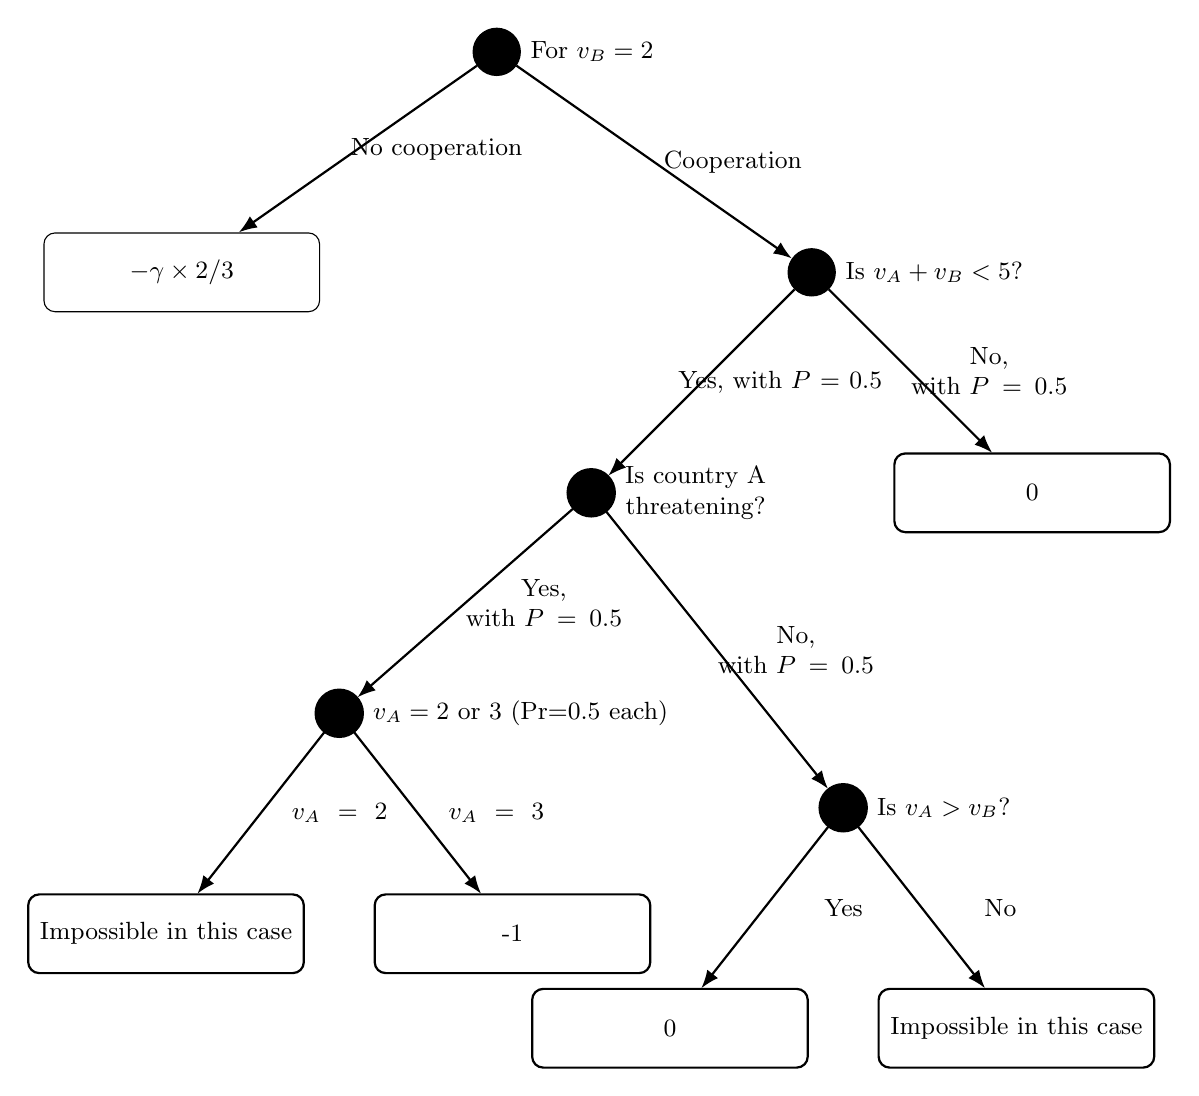
\begin{tikzpicture}[
    scale=0.8, 
  grow=down,
  level 1/.style={sibling distance=10cm, level distance=3.5cm},
  level 2/.style={sibling distance=7cm, level distance=3.5cm},
  level 3/.style={sibling distance=8cm, level distance=3.5cm},
  level 4/.style={sibling distance=5.5cm, level distance=3.5cm},
  edge from parent/.style={draw, -{Latex}, thick},
  every node/.style={font=\small, align=center},
  decision/.style={circle, draw, fill=black, inner sep=1.5pt, minimum size=6mm},
  terminal/.style={rectangle, draw, inner sep=2pt, rounded corners, minimum width=3.5cm, minimum height=1cm},
  edge label/.style={font=\small, align=center, midway, xshift=1cm, text width=3cm}
]

\node[decision, label=right:{For $v_B=2$}] {}
  child {
    node[terminal] {$-\gamma \times 2/3$}
    edge from parent node[edge label] {No cooperation}
  }
  child {
    node[decision, label=right:{Is $v_A + v_B < 5$?}] {}
    child {
      node[decision, label=right:{Is country A \\ threatening?}] {}
      child {
        node[decision, label=right:{$v_A=2$ or $3$ (Pr=0.5 each)}] {}
        child {
          node[terminal] {Impossible in this case}
          edge from parent node[edge label] {$v_A=2$}
        }
        child {
          node[terminal] {-1}
          edge from parent node[edge label] {$v_A=3$}
        }
        edge from parent node[edge label] {Yes,\\ with $P=0.5$}
      }
      child [level distance=5cm] {
        node[decision, label=right:{Is $v_A > v_B$?}] {}
        child {
          node[terminal] {0}
          edge from parent node[edge label] {Yes}
        }
        child {
          node[terminal] {Impossible in this case}
          edge from parent node[edge label] {No}
        }
        edge from parent node[edge label] {No,\\ with $P=0.5$}
      }
      edge from parent node[edge label] {Yes, with $P=0.5$}
    }
    child {
      node[terminal] {0}
      edge from parent node[edge label] {No,\\ with $P=0.5$}
    }
    edge from parent node[edge label] {Cooperation}
  };

\end{tikzpicture}
\end{center}

% ------------------------------------------------------------------

\subsubsubsection{Case: $v_B = 3$}


\paragraph{Analytical Resolution}

\textbf{Expected Utility of Not Cooperating}

We compute:

\[
= -\gamma \times 3 \times \Pr(d_A > 4 - 3)
= -\gamma \times 3 \times \frac{2}{3}
= -2\gamma.
\]

\textbf{Expected Utility of Cooperating}

We compute:

\begin{align*}
&\underbrace{
    \Pr(\text{A threatening}) \times \Pr(v_A = 3) \times (-2)
}_{\text{if A threatens and $v_A = 3$ (has to choose db=vb-2)}}
\\[3ex]
&+
\underbrace{
    \Pr(\text{A threatening}) \times \Pr(v_A = 2) \times (-1)
}_{\text{if A threatens and $v_A = 2$ (has to choose db=vb-1)}}
\\[3ex]
&+
\underbrace{
    \Pr(\text{non-threatening}) \times \frac{1}{2} \times \Pr(v_A = v_B) \times (-1)
}_{\text{equal debt level: effort -1}}
\\[3ex]
&+
\underbrace{
    \Pr(\text{non-threatening}) \times \frac{1}{2} \times \Pr(v_A > v_B) \times (-1)
}_{\text{A has more debt: effort -1}}.
\end{align*}

Plugging in the values:

\[
= 0.5 \times 0.5 \times (-2)
+ 0.5 \times 0.5 \times (-1)
+ 0.5 \times 0.5 \times 0.5 \times (-1)
+ 0.5 \times 0.5 \times 0.5 \times (-1)
\]

We simplify:

\[
= (0.25 \times -2)
+ (0.25 \times -1)
+ (0.125 \times -1)
+ (0.125 \times -1)
\]

\[
= -0.5 - 0.25 - 0.125 - 0.125 = -1.
\]

\paragraph{Interpretation}

\begin{itemize}
    \item If $\gamma \geq 0.5$, cooperating is better than not cooperating (because $-1 > -2\gamma$ when $\gamma > 0.5$).
    \item If $\gamma < 0.5$, not cooperating is preferable.
\end{itemize}

\paragraph{Decision Tree}
\begin{center}
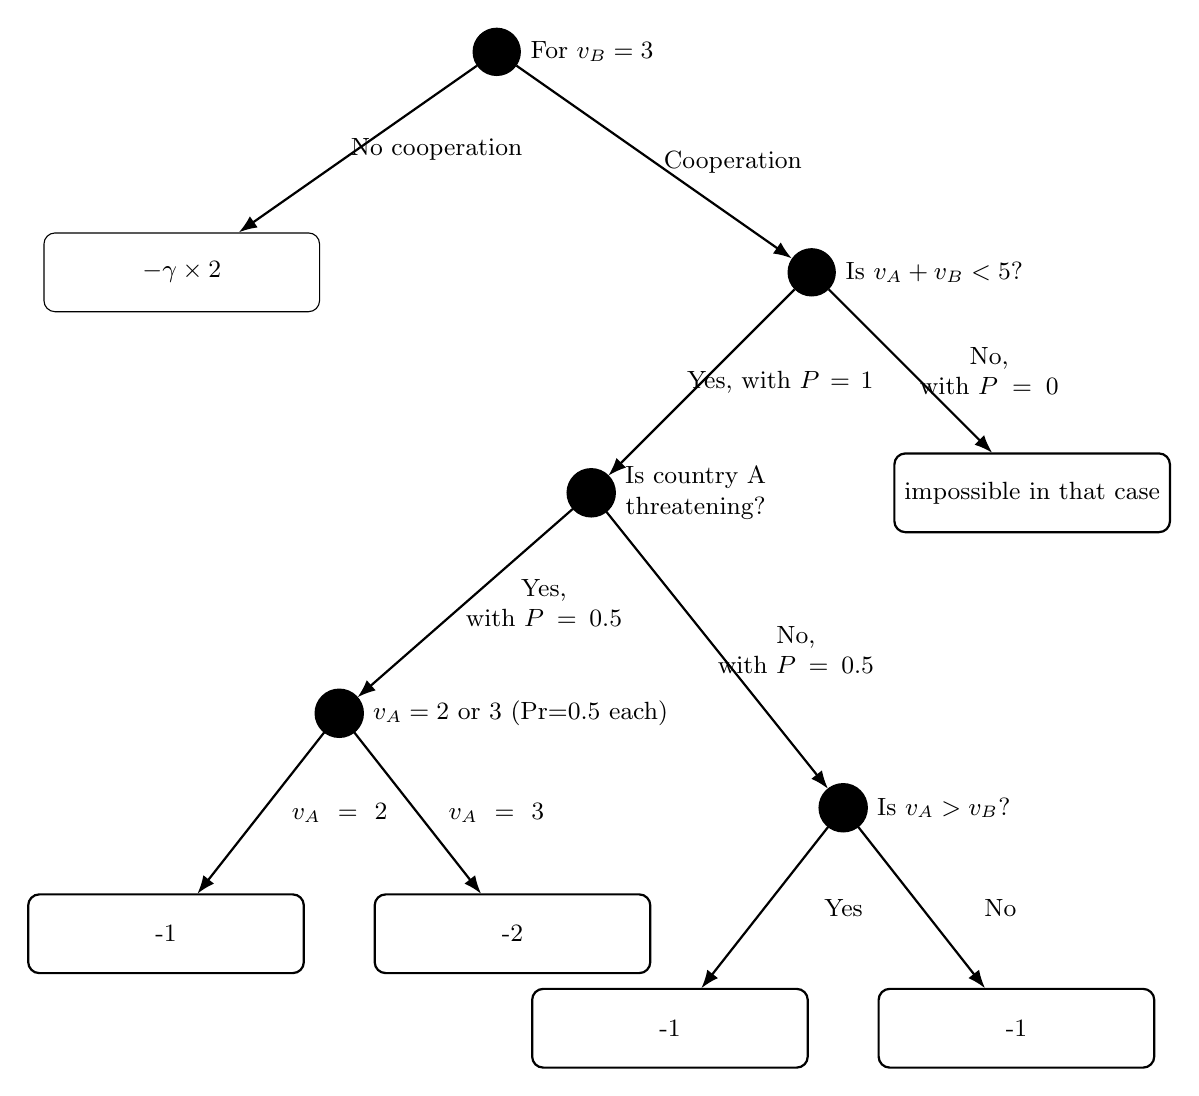
\begin{tikzpicture}[
    scale=0.8, 
  grow=down,
  level 1/.style={sibling distance=10cm, level distance=3.5cm},
  level 2/.style={sibling distance=7cm, level distance=3.5cm},
  level 3/.style={sibling distance=8cm, level distance=3.5cm},
  level 4/.style={sibling distance=5.5cm, level distance=3.5cm},
  edge from parent/.style={draw, -{Latex}, thick},
  every node/.style={font=\small, align=center},
  decision/.style={circle, draw, fill=black, inner sep=1.5pt, minimum size=6mm},
  terminal/.style={rectangle, draw, inner sep=2pt, rounded corners, minimum width=3.5cm, minimum height=1cm},
  edge label/.style={font=\small, align=center, midway, xshift=1cm, text width=3cm}
]

\node[decision, label=right:{For $v_B=3$}] {}
  child {
    node[terminal] {$-\gamma \times 2$}
    edge from parent node[edge label] {No cooperation}
  }
  child {
    node[decision, label=right:{Is $v_A + v_B < 5$?}] {}
    child {
      node[decision, label=right:{Is country A \\ threatening?}] {}
      child {
        node[decision, label=right:{$v_A=2$ or $3$ (Pr=0.5 each)}] {}
        child {
          node[terminal] {-1}
          edge from parent node[edge label] {$v_A=2$}
        }
        child {
          node[terminal] {-2}
          edge from parent node[edge label] {$v_A=3$}
        }
        edge from parent node[edge label] {Yes,\\ with $P=0.5$}
      }
      child [level distance=5cm] {
        node[decision, label=right:{Is $v_A > v_B$?}] {}
        child {
          node[terminal] {-1}
          edge from parent node[edge label] {Yes}
        }
        child {
          node[terminal] {-1}
          edge from parent node[edge label] {No}
        }
        edge from parent node[edge label] {No,\\ with $P=0.5$}
      }
      edge from parent node[edge label] {Yes, with $P=1$}
    }
    child {
      node[terminal] {impossible in that case}
      edge from parent node[edge label] {No,\\ with $P=0$}
    }
    edge from parent node[edge label] {Cooperation}
  };

\end{tikzpicture}
\end{center}



\subsection{Key Takeaways}

Country A will be more eager to cooperate than country B, and will need a lower punishment to be incentivized to do so. 
Both countries have a higher interest to cooperate with a higher debt, with this structure of punishment. 


The most interesting conclusion lies in the structure of the punishment chosen by the EC. 
We notice for country B that it has more incentive to cooperate $$(3/8 < 1/2)$$ when it has a high debt, but that's linked to the proportional nature of the EC punishment. 
If the EC was only inflicting a fixed cost $\gamma$, instead of $di \times \gamma$, we would have for $Vb=2$: 
\[
U_{\text{no cooperation}} = -\frac{1}{3} \gamma
\quad \text{and} \quad
U_{\text{cooperation}} = -\frac{1}{4}.
\]

\begin{itemize}
    \item If $\gamma \geq \dfrac{3}{4}$, colluding provides a higher expected utility for $Vb=2$.
\end{itemize}

For  $Vb=3$

\[
U_{\text{no cooperation}} = -\frac{2}{3} \gamma
\quad \text{and} \quad
U_{\text{cooperation}} = -1.
\]

\begin{itemize}
    \item If $\gamma \geq \dfrac{3}{2}$, colluding provides a higher expected utility for $Vb=3$.
\end{itemize}
\begin{simplebox}{Proposition 3.1}
   With fixed punishments, country B has less incentive to cooperate when it has more debt. This is linked to geopolitical risk: if country A can threaten you and make you drop your debt by 2 points, this is a huge decrease in utility. For a punishment small enough, you are better off being punished by the EC rather than having to enormlously decrease your debt.
\end{simplebox}


The EC has two factors determining its utility.  The first one is to avoid punishing the countries and give them the lightest punishments, in order to not become an unpopular political actor. The second one is to avoid the debt limit being crossed to prevent the intervention of the ECB. \\

Comparing the two punishment structures, we find that proportional sanctions allow the Commission to enforce the debt limit with a substantially lower punishment intensity than fixed sanctions. In our model, making penalties proportional to debt effectively lowers the $\gamma$-threshold needed to sustain cooperation, because each country internalizes more of the cost of excessive borrowing. By contrast, under fixed punishments the minimum $\gamma$ required to deter deviations is much higher – so high that it may be politically infeasible given the Commission’s aversion to draconian measures. This insight implies that a proportionate punishment scheme better aligns incentives: even without a “bang-bang” extreme sanction, both countries prefer to keep the total debt below the enforcement trigger when faced with proportional fines. Put simply, scaling penalties to each country’s debt burden lets the EC induce cooperation with a lighter touch, upholding the debt limit while avoiding the need for unreasonably harsh punishments.

We can thus draw the following policy conclusion: it's better for the EC to make the punishment proportional to the amount of debt taken rather than keeping it fixed. Indeed, we need a $\gamma$ much higher with fixed punishment to ensure cooperation between the two countries, and thus, the debt limit treshold being respected when they both want to take a lot of debt. By making this punishment proportional, the EC can thus choose a lower $\gamma$ and gain "popularity" compared to a fixed one. 



% ------------------------------------------------------------------

\section{Conclusion}

This paper has examined the strategic underpinnings of fiscal rule enforcement within the Eurozone, focusing on the interaction between member states and the European Commission (EC). Across three models of increasing complexity, we have shown how credibility, enforcement capacity, and multilateral dynamics shape fiscal behavior and the prevalence of hidden debt strategies.

In the baseline signaling game, we found that the EC's lack of credible enforcement mechanisms can create perverse incentives. When the EC either punishes all debt increases indiscriminately or fails to punish even clear violations, honest governments may be discouraged from transparent reporting, while dishonest ones are incentivized to hide their fiscal intentions. This suggests that enforcement without informational nuance can reduce fiscal discipline rather than strengthen it.

The first extension shows how a government's internal trade-off between transparency and concealment hinges on its belief about the EC's enforcement strategy. When the expected punishment is high but enforcement credibility is low, dishonest governments are more likely to hide debt. Conversely, honest governments may use transparent debt increases as a test of the EC’s stance. Importantly, the model predicts that, while increasing the size of the punishment can be tempting, if the punishment in question is rarely enforced it will not lead to a significant change in the behaviour of member countries. 

The second extension adds coordination between multiple countries and highlights why the type of punishment chosen by the EC matters. In a world with an uneven balance of powers between countries, proportional penalties allow the EC to reduce the intensity of the penalties needed to deter countries from breaching the debt treshold. The EC can then enforce fiscal rules at a lower political cost.

Our multi-country results also illuminate how the structure of punishments affects the EU’s enforcement capacity. They suggest that a sanction scheme calibrated to the scale of violations can significantly enhance enforcement credibility in a union of peers. In particular, proportional debt-based penalties reduce the threshold of enforcement intensity needed for compliance, allowing the Commission to uphold fiscal rules without wielding extreme punishments. By contrast, a fixed fine would need to be set so high to deter joint violations that it risks becoming politically unsustainable. These insights stress that aligning the punishment magnitude with each country’s contribution to the breach improves the EC’s ability to enforce fiscal rules, linking our theoretical findings to broader questions of how to design more resilient enforcement frameworks.

These insights lead to two main policy recommendations. First, increasing the EC’s audit and monitoring capacity is essential. If hidden debt can be reliably detected, transparent enforcement becomes more credible and more effective. Second, aligning penalties with the scale of fiscal violations—such as making sanctions proportional to the amount of hidden debt—can strengthen incentives for compliance while reducing the political cost of enforcement.

While our models offer a structured framework for understanding these dynamics, they rely on simplifying assumptions. Future work should explore richer action spaces, probabilistic enforcement, and the role of domestic political actors and financial markets in shaping fiscal behavior. It should especially explore other interactions that may shape the EC’s beliefs aside from the direct messages it receives from member countries. Lastly, empirical calibration of model parameters using real-world data could further enhance the policy relevance of our findings and guide the design of more credible and efficient enforcement regimes within the EU.

\section{References}

Alesina, A. and Sachs, J.D. (1988) ‘Political parties and the business cycle in the United States, 1948–1984’, Journal of Money, Credit and Banking, 20(1), pp. 63–82. 


Alesina, A. and Tabellini, G. (1990) ‘A positive theory of fiscal deficits and government debt’, Review of Economic Studies, 57(3), pp. 403–414. 


Besley, T. and Smart, M. (2007) ‘Fiscal restraints and voter welfare’, Journal of Public Economics, 91(3–4), pp. 755–773. 


Debrun, X. and Kumar, M.S. (2007) ‘Fiscal Rules, Fiscal Councils and All That: Commitment Devices, Signaling Tools or Smokescreens?’, in Banca d’Italia (ed.) Fiscal Policy: Current Issues and Challenges, Papers presented at the Banca d’Italia workshop, Perugia, 29–31 March 2007, pp. 479–512. 


Drazen, A. and Eslava, M. (2005) ‘Electoral Manipulation via Expenditure Composition: Theory and Evidence’, NBER Working Paper No. 11085, National Bureau of Economic Research, Cambridge, MA. 


Halac, M. and Yared, P. (2022) ‘Fiscal Rules and Discretion Under Limited Enforcement’, Econometrica, 90(5), pp. 2093–2127. 


Kirchsteiger, G. and Larch, M. (2023) ‘The enforcement dilemma of EU fiscal rules’, CEPR Discussion Paper No. 18304, CEPR Press, Paris \& London. 


Roubini, N. and Sachs, J.D. (1989) ‘Political and economic determinants of budget deficits in the industrial democracies’, European Economic Review, 33(5), pp. 903–933. 


Wijsman, S. and Crombez, C. (2017) ‘The political economy of enforcing fiscal rules’, Working Paper No. 565362, Department of Management, Strategy and Innovation, KU Leuven. 

Leblond, P. (2006), “The Political Stability and Growth Pact is Dead: Long Live the Economic Stability and Growth Pact”, Journal of Common Market Studies, 44 (5), pp. 969-990


\section{Appendix}

\subsection {The right punishment: Derivation for country A}

\subsubsection{Country A}

\subsubsubsection{Case: $v_A = 2$}

\paragraph{Analytical Resolution}

\textbf{Expected Value of Not Cooperating}

We compute:
\[
= -\gamma \times 2 \times \Pr(d_A > 4 - 2)
= -\gamma \times 2 \times \frac{1}{3}
= -\frac{2}{3}\gamma.
\]

\textbf{Expected Value of Cooperating}

We compute:

\begin{align*}
&\underbrace{
    0 \times \Pr(v_A = 2)
}_{\text{no punishment if $v_B = 2$}}
\\[3ex]
&+
\underbrace{
   \Pr(\text{Country A is threatening})
    \times (0)
}_{\text{If country A can threaten country B, it chooses $vb=db$}}
\\[3ex]
&+
\underbrace{
    \Pr(\text{non-threatening})
    \times \Pr(v_A > v_B)
    \times 0
}_{\text{$Pr(v_A > v_B)$ is equal to 1, that's why we don't include the other option }}.
\end{align*}

Plugging in the values:

\[
= 0 \times 0.5
+ 0.5 \times 0 
+ 0.5 \times 1 \times 0
= 0.
\]

Since $0> -\frac{2}{3}\gamma$ for $\gamma$ different from 0, country A will always choose to cooperate in this case.

\paragraph{Decision Tree}

\begin{center}
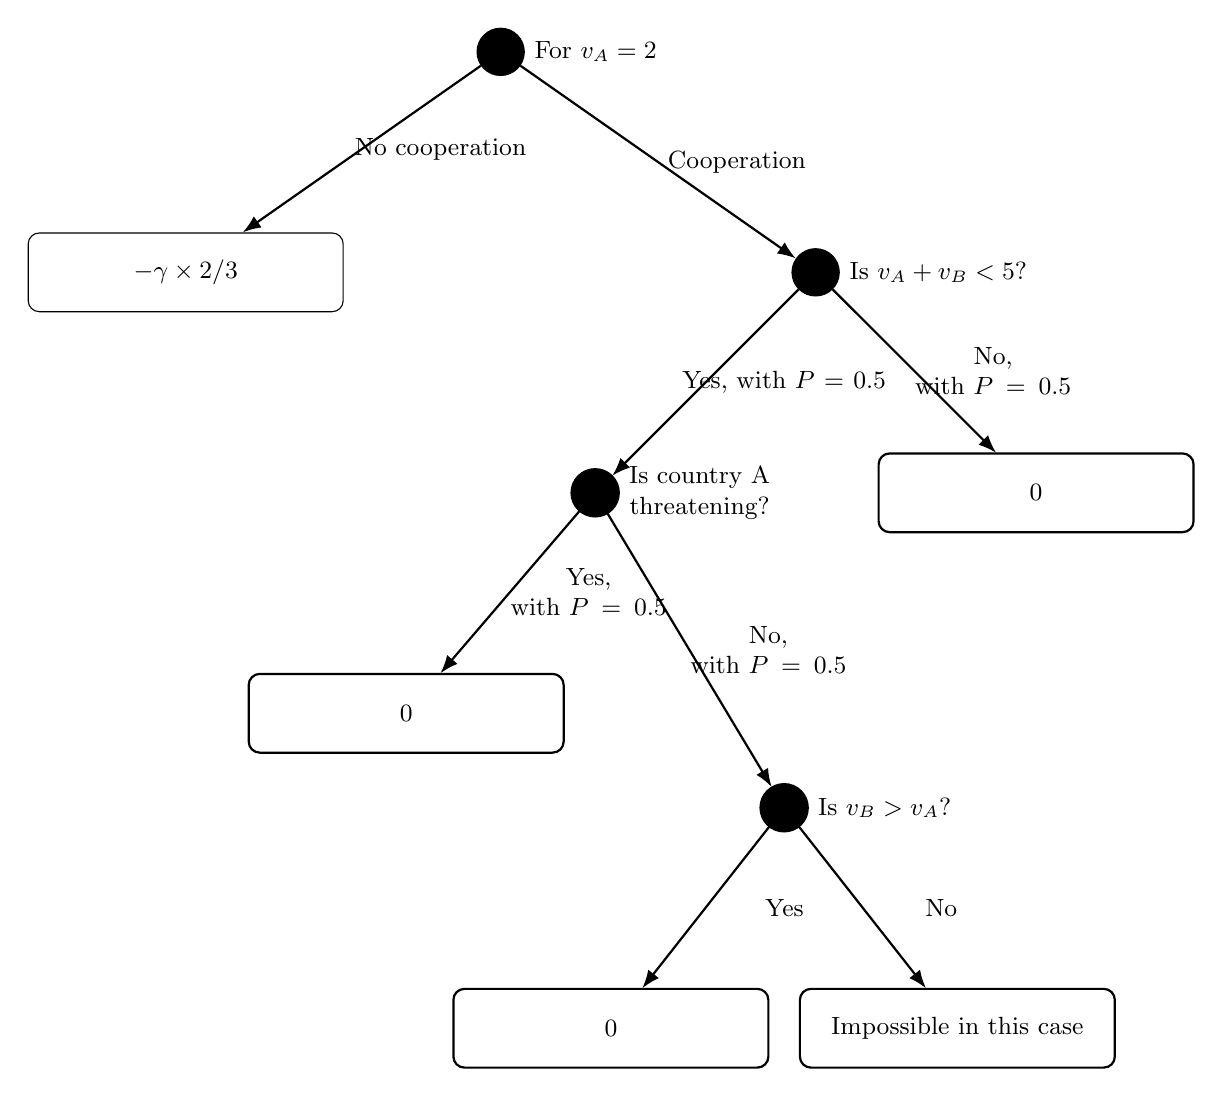
\begin{tikzpicture}[
    scale=0.8, 
  grow=down,
  level 1/.style={sibling distance=10cm, level distance=3.5cm},
  level 2/.style={sibling distance=7cm, level distance=3.5cm},
  level 3/.style={sibling distance=6cm, level distance=3.5cm},
  level 4/.style={sibling distance=5.5cm, level distance=3.5cm},
  edge from parent/.style={draw, -{Latex}, thick},
  every node/.style={font=\small, align=center},
  decision/.style={circle, draw, fill=black, inner sep=1.5pt, minimum size=6mm},
  terminal/.style={rectangle, draw, inner sep=2pt, rounded corners, minimum width=4cm, minimum height=1cm},
  edge label/.style={font=\small, align=center, midway, xshift=1cm, text width=3cm}
]

\node[decision, label=right:{For $v_A=2$}] {}
  child {
    node[terminal] {$-\gamma \times 2/3$}
    edge from parent node[edge label] {No cooperation}
  }
  child {
    node[decision, label=right:{Is $v_A + v_B < 5$?}] {}
    child {
      node[decision, label=right:{Is country A \\ threatening?}] {}
      child {
        node[terminal] {0}
        edge from parent node[edge label] {Yes,\\ with $P=0.5$}
      }
      child [level distance=5cm] {
        node[decision, label=right:{Is $v_B > v_A$?}] {}
        child {
          node[terminal] {0}
          edge from parent node[edge label] {Yes}
        }
        child {
          node[terminal] {Impossible in this case}
          edge from parent node[edge label] {No}
        }
        edge from parent node[edge label] {No,\\ with $P=0.5$}
      }
      edge from parent node[edge label] {Yes, with $P=0.5$}
    }
    child {
      node[terminal] {0}
      edge from parent node[edge label] {No,\\ with $P=0.5$}
    }
    edge from parent node[edge label] {Cooperation}
  };

\end{tikzpicture}
\end{center}

% ------------------------------------------------------------------

\subsubsubsection{Case: $v_A = 3$}

\paragraph{Analytical Resolution}

\textbf{Expected Utility of Not Cooperating}

We compute:

\[
= -\gamma \times 3 \times \Pr(d_A > 4 - 3)
= -\gamma \times 3 \times \frac{2}{3}
= -2\gamma.
\]

\textbf{Expected Utility of Cooperating}

We compute:

\begin{align*}
&\underbrace{
    \Pr(\text{A threatening}) \times 0
}_{\text{if A can threaten, it chooses $v_A = d_A$}}
\\[3ex]
&+
\underbrace{
    \Pr(\text{non-threatening}) \times \Pr(v_A = v_B) \times (-1)
}_{\text{equal debt level: effort -1}}
\\[3ex]
&+
\underbrace{
    \Pr(\text{non-threatening}) \times \Pr(v_A > v_B) \times (-1)
}_{\text{A has more debt: effort -1}}.
\end{align*}

Plugging in the values:

\[
= 0.5 \times 0 
+ 0.5 \times 0.5 \times (-1)
+ 0.5 \times 0.5 \times 0.5 \times (-1)
= -0.5
\]



\paragraph{Interpretation}

\begin{itemize}
    \item If $\gamma \geq 0.25$, cooperating is better than not cooperating.
    \item If $\gamma < 0.25$, not cooperating is preferable.
\end{itemize}


\paragraph{Decision Tree}

\begin{center}
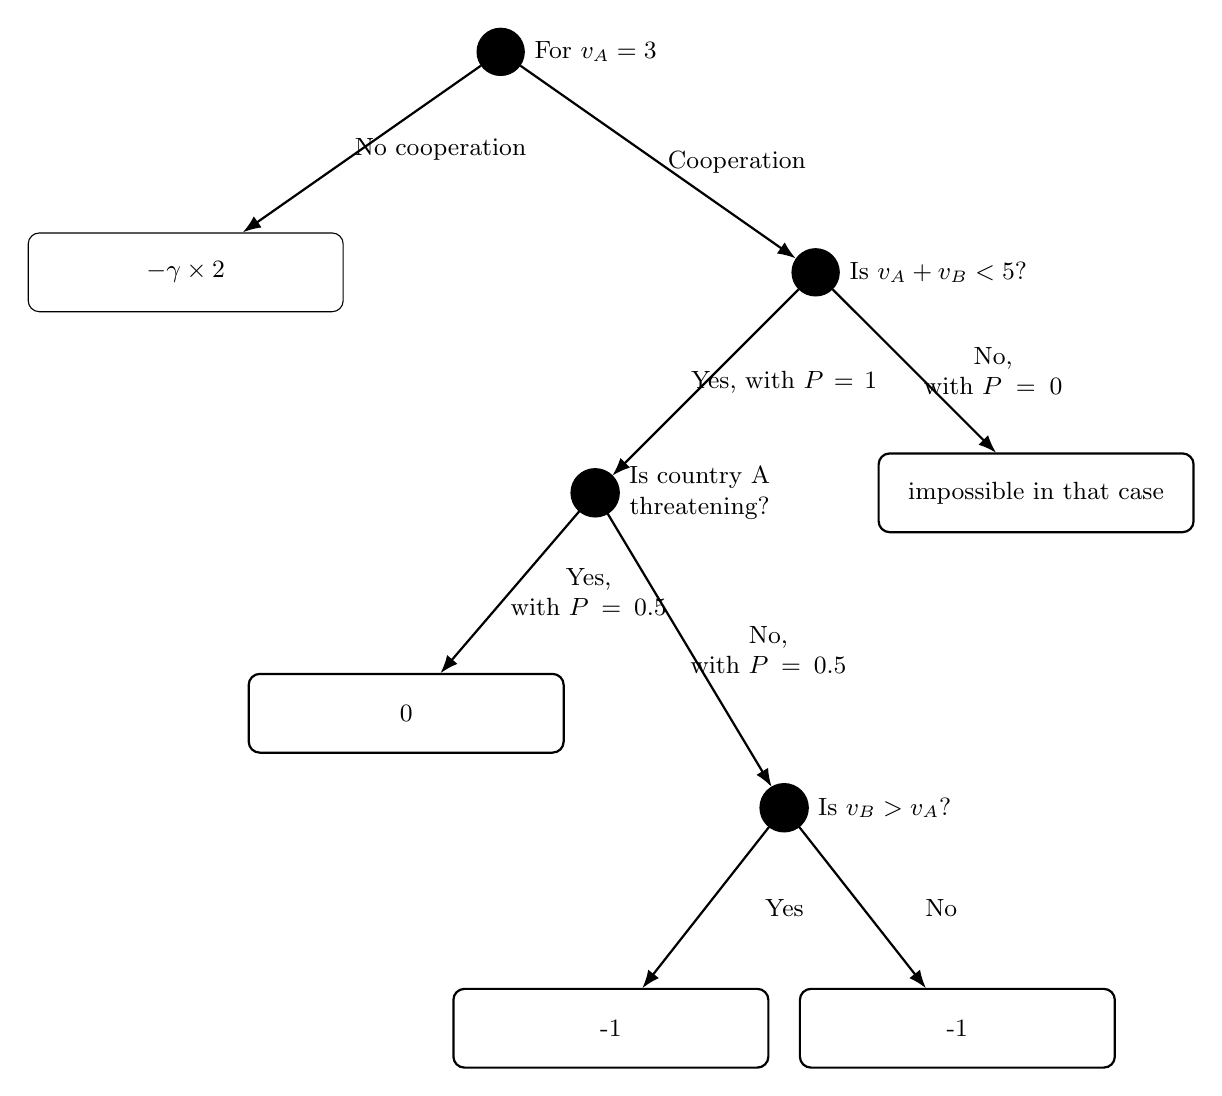
\begin{tikzpicture}[
    scale=0.8, 
  grow=down,
  level 1/.style={sibling distance=10cm, level distance=3.5cm},
  level 2/.style={sibling distance=7cm, level distance=3.5cm},
  level 3/.style={sibling distance=6cm, level distance=3.5cm},
  level 4/.style={sibling distance=5.5cm, level distance=3.5cm},
  edge from parent/.style={draw, -{Latex}, thick},
  every node/.style={font=\small, align=center},
  decision/.style={circle, draw, fill=black, inner sep=1.5pt, minimum size=6mm},
  terminal/.style={rectangle, draw, inner sep=2pt, rounded corners, minimum width=4cm, minimum height=1cm},
  edge label/.style={font=\small, align=center, midway, xshift=1cm, text width=3cm}
]

\node[decision, label=right:{For $v_A=3$}] {}
  child {
    node[terminal] {$-\gamma \times 2$}
    edge from parent node[edge label] {No cooperation}
  }
  child {
    node[decision, label=right:{Is $v_A + v_B < 5$?}] {}
    child {
      node[decision, label=right:{Is country A \\ threatening?}] {}
      child {
        node[terminal] {0}
        edge from parent node[edge label] {Yes,\\ with $P=0.5$}
      }
      child [level distance=5cm] {
        node[decision, label=right:{Is $v_B > v_A$?}] {}
        child {
          node[terminal] {-1}
          edge from parent node[edge label] {Yes}
        }
        child {
          node[terminal] {-1}
          edge from parent node[edge label] {No}
        }
        edge from parent node[edge label] {No,\\ with $P=0.5$}
      }
      edge from parent node[edge label] {Yes, with $P=1$}
    }
    child {
      node[terminal] {impossible in that case}
      edge from parent node[edge label] {No,\\ with $P=0$}
    }
    edge from parent node[edge label] {Cooperation}
  };

\end{tikzpicture}
\end{center}



\subsection{A Recursive Collaboration game}
\subsubsection{Principle}
The goal of the game mentioned below is to understand how the EC's reaction may change when countries decide to jointly increase their debt to push the EC to cower away from punishing anyone. In other words, when countries band together they can push the EC to be more lenient as the individual political cost of punishment is inflated by the number of countries increasing debt at once. Indeed, if there are multiple countries which choose to openly increase their debt at the same time, punishing even one country gets harder as undisciplined countries come to each other's help as evidenced by the case of France and Germany in 2003 (Leblond, 2006).
Another objective we had in mind when designing this game is to introduce a game that plays before the signaling game and influences both 1) the payoffs of the signaling game and 2) the belief of the EC about the type of each country. Regarding the latter, it is true that in reality the EC is not blind to actions that are taken by Italy outside of its decision to communicate an increase or not. The EC will always seek to update the prior probability is has for dishonesty based on unrelated interactions that may give away information about the type of a country. 
\subsubsection{Set-Up:}
\begin{itemize}
    \item 1 period game
    \item \underline{3 players :} country A, country B and the European Commission 
    \begin{enumerate}
        \item Country A and country B represent governments of member countries that wish to increase their debt as part of their domestic agenda. Under certain circumstances they will wish to collaborate with one another (coordinate their increase in debt) to reduce the odds of an action from the European Commission. If they do not collaborate they may choose to communicate either "no debt increase" or "debt increase" (similar to previous game) individually.
        As was the case in the base game, a dishonest country has the option between playing superbonus (hidden debt increase) and playing a transparent debt increase. Whereas, an honest country chooses between a transparent debt increase or no debt increase.
        \item European Commission : as a political institution, the European commission cares both for social welfare and its reputation amongst member countries. While it values stability and wishes to be seen as a credible institution (especially by members that take their debt level seriously), punishing a country might come with significant enforcement costs if the decision is unpopular. It interacts with each country independently and can choose to punish Country A, country B, both countries or none. 
    \end{enumerate}
    \item \underline{How the game unfolds : }
    \begin{enumerate}
        \item Stage 1 : Nature draws the type $\theta_A$ of country A and $\theta_B$ of country B separately via a Bernoulli distribution of parameter $\mu_A$ ($\mu_B$ respectively). These types remain private (they are not revealed to the other country or to the EC). When considering $\mu_A\neq \mu_B$ this can serve to model cases where countries have different histories in terms of public spending. 
        \item Stage 2 (simultaneous) : Each countries decides on which message it will communicate ($m_{debt},m_{nodebt}$) to the EC while taking into account what the other one will do. If both choose $m_{debt}$ we consider there is collaboration which will affect the enforcement costs for the EC. Otherwise, they are on their own. 
        \item Stage 3 (sequential): The EC observes the message sent by member countries and whether they decided to collaborate. It decides on an individual basis whether it will punish each country. We then consider its aggregate utility after having taken a decision for both countries. 
    \end{enumerate}
\end{itemize}

\subsubsection{Visualizing the game}
\textbf{Stage 1 : Type draw }
Types are drawn for country A and B with : 
\begin{equation}
\left\{
\begin{aligned}
    &\theta_A\sim Ber(\mu_A) \text{ and } \theta_B\sim Ber(\mu_B)\\
    &P(\theta_A=\theta_{A,H}) = \mu_A \text{ and } P(\theta_B=\theta_{B,H}) = \mu_B\\
    &P(\theta_A=\theta_{A,D}) =  1-\mu_A \text{ and } P(\theta_B=\theta_{B,D}) = 1-\mu_B
\end{aligned}
\right.
\end{equation}
\textbf{Stage 2 : Collaboration game - simultaneous}
We assume the following (which might be challenged when deriving the model) : with $D_{nocoll}\equiv D$
\begin{itemize}
    \item $S-P<S^{coll}<S$
    \item $c<R<2c$
    \item the type of each player is unknown to the other
\end{itemize}
The countries decide on which message they are going to send to the EC while accounting for what the other will send. If both choose to communicate an increase in debt, they collaborate to have a better chance of it passing and communicate about their alliance to the EC (otherwise would not impact its payoff). 
\begin{table}[H]
$\begin{array}{c|cc}  
\text{Country A} \backslash \text{Country B} & m_{debt} & m_{nodebt} \\   
\hline   
m_{debt} & U_A(m_{debt}^{coll});U_B(m_{debt}^{coll}) & U_A(m_{debt});U_B(m_{nodebt}|\theta_B)\\  
m_{nodebt} & U_A(m_{nodebt}|\theta_A),U_B(m_{debt})& U_A(m_{nodebt}|\theta_A), U_B(m_{nodebt}|\theta_B) 
\end{array}$  
\caption{Payoff Matrix for the collusion game}  
\label{tab:payoff_matrix}  
\end{table}  

\textbf{Detailed payoffs :}
\begin{itemize}
    \item \underline{Collaboration case :} $\forall_i\in[A,B], U_i(m_{debt}^{coll})=S^{coll}$ (the gain is guaranteed since the cost of punishment for the EC is too high as will be described below)
    \item \underline{No collaboration case:} $\forall_i\in[A,B]$
    \begin{enumerate}
        \item communicate debt : (not dependent on type as communicating an increase in debt is a transparent action $\Rightarrow$ punishment is automatic since we assumed $R>c$) 
        \begin{equation}
        \begin{aligned}
            U_i(m_{debt})=(S-P)
        \end{aligned}
        \end{equation}
        \item communicate no debt : we note $\theta_{i,H}$ to indicate that country i is of the honest type. 
        \begin{equation}  
        \begin{aligned}  
            &U_i(m_{\text{nodebt}} \mid \theta_{i,H}) = P(\text{EC}(P) \mid m_{\text{nodebt}})\times(- P) + P(\text{EC}(NP) \mid m_{\text{nodebt}}) \times 0   \\  
            &U_i(m_{\text{nodebt}} \mid \theta_{i,D}) =   
                \underbrace{P(\text{EC}(P) \mid m_{\text{nodebt}})}_{  
                    \substack{  
                        \text{probability that the EC will} \\  
                        \text{punish when receiving } m_{\text{nodebt}}  
                    }  
                }\times(S - P) + P(\text{EC}(NP) \mid m_{\text{nodebt}}) \times S  
        \end{aligned}  
        \end{equation}  
    \end{enumerate}
\end{itemize}

\noindent\textbf{Stage 3 : Signaling game - sequential}\\
\textbf{Country A and B \textcolor{red}{colluded}:} the enforcement cost for the EC goes up and we have the following for both country and country B: 

\begin{center}  
  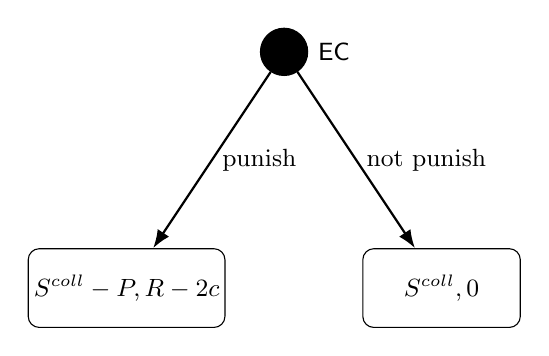
\begin{tikzpicture}[  
      grow=down,  % Changed from right to up  
      level distance=3cm,  
      sibling distance=4cm,  
      edge from parent/.style={draw, -{Latex}, thick},  
      every node/.style={font=\sffamily\small},  
      decision/.style={circle, draw, fill=black, inner sep=1.5pt, minimum size=6mm},  
      terminal/.style={rectangle, draw, inner sep=2pt, rounded corners, minimum width=2cm, minimum height=1cm}  
    ]  
    % Root node: EC decision  
    \node[decision, label=right:{EC}] {}  % Changed label from above to right  
      child {  
        node[terminal] {$S^{coll}-P,R-2c$}  
          edge from parent node[right, font=\small]{punish}  % Changed from above to right  
      }  
      child {  
        node[terminal] {$S^{coll},0$}  
          edge from parent node[right, font=\small]{not punish}  % Changed from above to right  
      };  
  \end{tikzpicture}  
\end{center} 
Basically, he EC faces twice the enforcement cost if it wishes to punish either of the two countries (It is as if it were taking the loss for punishing both countries but with half the gains). \\[1em] 
\textbf{Country A and B \textcolor{red}{did not collude }: } Each player plays the action it decided to play in stage 2 and the EC faces the following
\begin{itemize}
    \item If observes $m_{debt}$ : no uncertainty on the ideal action to take. It is worthwhile to punish regardless of type as long as $R>c$ which we assulmed above. 
\begin{center}  
  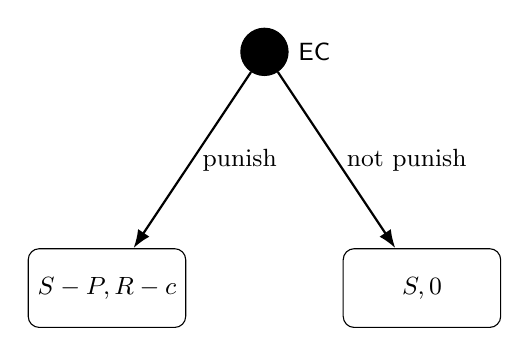
\begin{tikzpicture}[  
      grow=down,  % Changed from right to up  
      level distance=3cm,  
      sibling distance=4cm,  
      edge from parent/.style={draw, -{Latex}, thick},  
      every node/.style={font=\sffamily\small},  
      decision/.style={circle, draw, fill=black, inner sep=1.5pt, minimum size=6mm},  
      terminal/.style={rectangle, draw, inner sep=2pt, rounded corners, minimum width=2cm, minimum height=1cm}  
    ]  
    % Root node: EC decision  
    \node[decision, label=right:{EC}] {}  % Changed label from above to right  
      child {  
        node[terminal] {$S-P,R-c$}  
          edge from parent node[right, font=\small]{punish}  % Changed from above to right  
      }  
      child {  
        node[terminal] {$S,0$}  
          edge from parent node[right, font=\small]{not punish}  % Changed from above to right  
      };  
  \end{tikzpicture}  
\end{center} 
    \item If observes $m_{nodebt}$ : still faces uncertainty whether you are honest or dishonest (honest case to the left and dishonest case to the tree) so might hesitate to punish even though $S>c$. 

\begin{center}  
  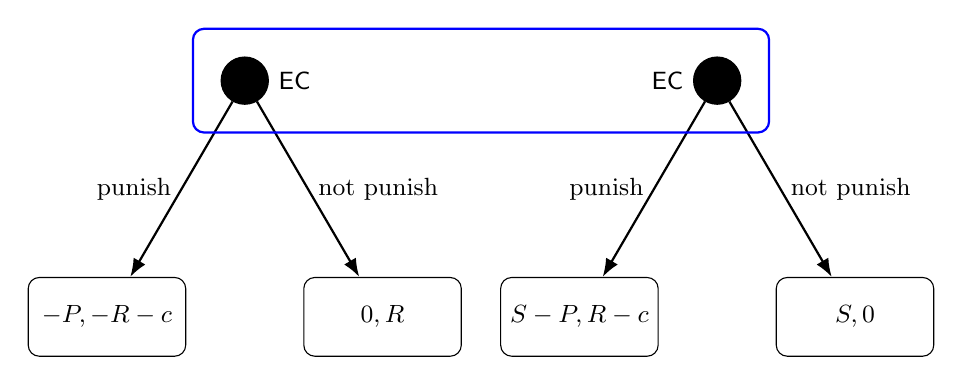
\begin{tikzpicture}[  
      grow=down,  
      level distance=3cm,  
      sibling distance=3.5cm,  % Keeps the wider spacing  
      edge from parent/.style={draw, -{Latex}, thick},  
      every node/.style={font=\sffamily\small},  
      decision/.style={circle, draw, fill=black, inner sep=1.5pt, minimum size=6mm},  
      terminal/.style={rectangle, draw, inner sep=2pt, rounded corners, minimum width=2cm, minimum height=1cm}  
    ]  
    % First tree shifted left:  
    \node[decision, label=right:{EC}] (EC1) at (-3,0) {}  
      child {  
        node[terminal] {$-P,-R-c$}  
          edge from parent node[left, font=\small]{punish}  
      }  
      child {  
        node[terminal] {$0,R$}  
          edge from parent node[right, font=\small]{not punish}  
      };  
  
    % Second tree shifted right:  
    \node[decision, label=left:{EC}] (EC2) at (3,0) {}  
      child {  
        node[terminal] {$S-P,R-c$}  
          edge from parent node[left, font=\small]{punish}  
      }  
      child {  
        node[terminal] {$S,0$}  
          edge from parent node[right, font=\small]{not punish}  
      };  
  
    % Blue box with just outline, no fill  
    \node[draw=blue, rounded corners, thick, inner sep=10pt, fit=(EC1) (EC2)] {};  
      
  \end{tikzpicture}  
\end{center}  
\subsubsection{Perspectives and limitations}
This game is difficult to solve as there a strong cyclical aspect to it : the action taken in stage 1 influences both the payoffs in the second stage and the beliefs that the Commission has about country types. However, this since the beliefs of the commission change, so will the expected utilities of country A and B which will affect their decisions in stage 1. While we hypothesize a solution could be found by fixing the action of a dishonest country in stage 1 and proceed to find a fixed point using an algorithm, we did not manage to find a convincing solution to this model. 
One way the solvability of this model could be significantly improved is by making sure the first game is disconnected from payoffs in the second game, save through the additional bayesian updating done by the EC as it observes the outcome of the first game. Nonetheless, this would imply finding another way to reproduce the tradeoff between colluding and getting less debt for sure and facing the EC on your own and risk being punished. 
    
\end{itemize}

\subsection{Code}
\subsubsection{3D graph}
\begin{lstlisting}[style=R]  

install.packages("plotly")

gamma_vals <- seq(0.01, 0.99, length.out = 40)
P_vals <- seq(0.1, 1.0, length.out = 40)
mu_vals <- seq(0.1, 0.99, by = 0.05)

surface_list <- lapply(mu_vals, function(mu_val) {
  grid <- expand.grid(gamma = gamma_vals, P = P_vals)
  grid$f <- with(grid, P * (gamma - 1) / ((mu_val - 1) * (1 + gamma)))
  f_matrix <- matrix(grid$f, nrow = length(P_vals), ncol = length(gamma_vals))
  list(z = f_matrix, mu = mu_val)
})

surface_list[[1]]$z[1:6, 1:6]

library(plotly)

frames <- lapply(seq_along(mu_vals), function(i) {
  list(
    data = list(
      list(
        x = gamma_vals,
        y = P_vals,
        z = surface_list[[i]]$z,
        type = 'surface',
        colorscale = 'Jet',
        showscale = TRUE
      )
    ),
    name = as.character(mu_vals[i])
  )
})

fig <- plot_ly(
  x = ~gamma_vals, y = ~P_vals, z = ~surface_list[[1]]$z,
  type = 'surface',
  colorscale = 'Jet',
  showscale = TRUE
)

fig <- fig %>% layout(
  scene = list(
    xaxis = list(title = 'gamma'),
    yaxis = list(title = 'P'),
    zaxis = list(title = 'H*')
  ),
  title = 'Interactive 3D Surface Plot of f(gamma, mu, P) with mu Slider',
  sliders = list(
    list(
      active = 0,
      currentvalue = list(prefix = 'mu = '),
      pad = list(t = 50),
      steps = lapply(seq_along(mu_vals), function(i) {
        list(
          method = 'animate',
          args = list(list(as.character(mu_vals[i])), list(mode = 'immediate', frame = list(duration = 500, redraw = TRUE), transition = list(duration = 0))),
          label = as.character(mu_vals[i])
        )
      })
    )
  )
)

fig$x$frames <- frames
fig

\end{lstlisting}  


\subsubsection{Monotone Comparative statics graphs}
\begin{lstlisting}[style=R]  

library(ggplot2)  
if (!requireNamespace("patchwork", quietly = TRUE)) {  
  install.packages("patchwork", repos="https://cran.rstudio.com/")  
}  
library(patchwork)  

# Define parameter ranges and representative values  
mu_seq <- seq(0.1, 0.99, length.out = 200)  
gamma_seq <- seq(0.01, 0.99, length.out = 200)  
P_seq <- seq(0.1, 10, length.out = 200)  
gamma_vals <- c(0.2, 0.5, 0.8)  
mu_vals <- c(0.2, 0.5, 0.8)  
P_vals <- c(0.5, 1, 2)  

get_ylim <- function(y) {  
  q <- quantile(y, probs = c(0.01, 0.99), na.rm = TRUE)  
  c(q[1], q[2])  
}  

# 1. ∂f/∂P vs μ for several γ  
plot1_data <- do.call(rbind, lapply(gamma_vals, function(gamma) {  
  data.frame(  
    mu = mu_seq,  
    dfdP = (gamma - 1) / ((mu_seq - 1) * (1 + gamma)),  
    gamma = as.factor(gamma)  
  )  
}))  
p1 <- ggplot(plot1_data, aes(x = mu, y = dfdP, color = gamma)) +  
  geom_line(linewidth = 1) +  
  labs(title = "∂f/∂P vs μ ", x = expression(mu), y = expression(partialdiff*f/P), color = expression(gamma)) +  
  theme_minimal() +  
  coord_cartesian(ylim = get_ylim(plot1_data$dfdP))  

# 2. ∂f/∂γ vs μ for several P (γ = 0.5)  
plot2_data <- do.call(rbind, lapply(P_vals, function(P) {  
  gamma <- 0.5  
  data.frame(  
    mu = mu_seq,  
    dfdgamma = P * ((mu_seq - 1) - (gamma - 1)) / ((mu_seq - 1) * (1 + gamma)^2),  
    P = as.factor(P)  
  )  
}))  
p2 <- ggplot(plot2_data, aes(x = mu, y = dfdgamma, color = P)) +  
  geom_line(linewidth = 1) +  
  labs(title = "∂f/∂γ vs μ (γ=0.5)", x = expression(mu), y = expression(partialdiff*f/gamma), color = "P") +  
  theme_minimal() +  
  coord_cartesian(ylim = get_ylim(plot2_data$dfdgamma))  

# 3. ∂f/∂μ vs γ for several P (μ = 0.5)  
plot3_data <- do.call(rbind, lapply(P_vals, function(P) {  
  mu <- 0.5  
  data.frame(  
    gamma = gamma_seq,  
    dfdmu = -P * (gamma_seq - 1) / ((1 + gamma_seq) * (mu - 1)^2),  
    P = as.factor(P)  
  )  
}))  
p3 <- ggplot(plot3_data, aes(x = gamma, y = dfdmu, color = P)) +  
  geom_line(linewidth = 1) +  
  labs(title = "∂f/∂μ vs γ (μ=0.5)", x = expression(gamma), y = expression(partialdiff*f/mu), color = "P") +  
  theme_minimal() +  
  coord_cartesian(ylim = get_ylim(plot3_data$dfdmu))  

# 4. ∂f/∂P vs γ for several μ  
plot4_data <- do.call(rbind, lapply(mu_vals, function(mu) {  
  data.frame(  
    gamma = gamma_seq,  
    dfdP = (gamma_seq - 1) / ((mu - 1) * (1 + gamma_seq)),  
    mu = as.factor(mu)  
  )  
}))  
p4 <- ggplot(plot4_data, aes(x = gamma, y = dfdP, color = mu)) +  
  geom_line(linewidth = 1) +  
  labs(title = "∂f/∂P vs γ", x = expression(gamma), y = expression(partialdiff*f/P), color = expression(mu)) +  
  theme_minimal() +  
  coord_cartesian(ylim = get_ylim(plot4_data$dfdP))  

# 5. ∂f/∂μ vs P for several γ (μ = 0.5)  
plot5_data <- do.call(rbind, lapply(gamma_vals, function(gamma) {  
  mu <- 0.5  
  data.frame(  
    P = P_seq,  
    dfdmu = -P_seq * (gamma - 1) / ((1 + gamma) * (mu - 1)^2),  
    gamma = as.factor(gamma)  
  )  
}))  
p5 <- ggplot(plot5_data, aes(x = P, y = dfdmu, color = gamma)) +  
  geom_line(linewidth = 1) +  
  labs(title = "∂f/∂μ vs P (μ=0.5)", x = "P", y = expression(partialdiff*f/mu), color = expression(gamma)) +  
  theme_minimal() +  
  coord_cartesian(ylim = get_ylim(plot5_data$dfdmu))  

# 6. ∂f/∂γ vs P for several μ (γ = 0.5)  
plot6_data <- do.call(rbind, lapply(mu_vals, function(mu) {  
  gamma <- 0.5  
  data.frame(  
    P = P_seq,  
    dfdgamma = P_seq * ((mu - 1) - (gamma - 1)) / ((mu - 1) * (1 + gamma)^2),  
    mu = as.factor(mu)  
  )  
}))  
p6 <- ggplot(plot6_data, aes(x = P, y = dfdgamma, color = mu)) +  
  geom_line(linewidth = 1) +  
  labs(title = "∂f/∂γ vs P (γ=0.5)", x = "P", y = expression(partialdiff*f/gamma), color = expression(mu)) +  
  theme_minimal() +  
  coord_cartesian(ylim = get_ylim(plot6_data$dfdgamma))  

# Arrange all six plots in a 2x3 grid
(p4 | p2 | p1) /  
  (p6 | p3 | p5)  
\end{lstlisting}  

\end{document}   


